\documentclass[a4paper,11pt]{article}

\usepackage[utf8]{inputenc}
\usepackage[T1]{fontenc}
\usepackage[french]{babel}
\usepackage{bm}

\usepackage{amsmath, amssymb}
\usepackage{graphicx}
\usepackage{float}
\usepackage[hidelinks]{hyperref}

\usepackage{geometry}
\geometry{margin=2cm}

\usepackage{listings}
\usepackage{xcolor}


\title{Report - Image Restoration by Inverse Problem with Kernel Estimation}
\author{Rothlingshofer Yanic, Douar Lounes}


\begin{document}

\begin{titlepage}
    \thispagestyle{empty}
    
    \noindent
    
\includegraphics[width=0.2\textwidth]{../figures/logo_TP.png}
    
    \vspace{2cm}
    
    \begin{center}
        {\LARGE \textbf{Image Restoration by Inverse Problem}}\\[0.3cm]
        {\LARGE \textbf{with Kernel Estimation}}\\[1cm]
        
        {\Large Final Report}\\[1.5cm]
    \end{center}
    
    \begin{flushleft}
        \textbf{Date :} 16/11/2025\\[0.3cm]
        \textbf{Students :} Rothlingshofer Yanic, Douar Lounes\\[0.3cm]
        \textbf{Supervisor :} Saïd Ladjal\\[0.3cm]
        \textbf{School :} Télécom Paris\\[0.3cm]
        \textbf{Course :} CSC\_4IM01\_TP\\[0.3cm]
        \textbf{Code :} \url{https://github.com/yrothlin-03/PROJ_IM01/tree/main}
    \end{flushleft}
    
    \vfill
\end{titlepage}
  
\setcounter{page}{1}

\section{Introduction}

Cameras and photographic equipment overall have seen significant improvements over the last decades.
However, capturing high-quality images in all conditions remains challenging, in particular in low-light situations where long exposure times are required and even small camera or scene motions lead to visible blur.
Image restoration and, more specifically, image deblurring have therefore been extensively studied.
Classical blind deconvolution methods explicitly model the image formation process as a convolution with an unknown point spread function (or blur kernel) and formulate its recovery in a Bayesian or maximum a posteriori (MAP) framework, combined with suitable priors on the latent sharp image such as heavy–tailed gradient or sparsity models, or variational regularisation terms \cite{MAP_bay,hyperlaplacian,hyperlap_blind}.
In parallel, most recent state-of-the-art approaches rely on deep neural networks trained on large datasets of blurred and sharp image pairs; these methods often achieve impressive performance but require substantial computational resources and large amounts of training data, and their internal representations are generally hard to interpret.

In this report, we deliberately follow a more traditional variational strategy and decouple the blur-kernel estimation from the image restoration.
First, we estimate the blur kernel from the blurred image by exploiting prior knowledge on natural image power spectra and on the effect of motion blur in the Fourier domain, following the Goldstein–Fattal framework as analysed by Anger et al. \cite{gf}.
This yields an approximation of the modulus of the kernel’s Fourier transform from which a spatial kernel can be reconstructed.
Then, assuming this kernel to be known, we perform a non-blind deconvolution in a variational setting with total variation (TV) regularisation, which we solve using the Split Bregman method \cite{goldsb,tvipol}.
This pipeline is fully interpretable, does not require any training data, and provides a simple variational baseline compared to more sophisticated Bayesian or hyper-Laplacian–prior blind-deblurring methods \cite{MAP_bay,hyperlaplacian,hyperlap_blind}.
In the following, we present the mathematical formulation of the problem, the kernel estimation method, and the results obtained with this approach.

\subsection{Mathematical model for deblurring}
Most image deblurring methods rely on a simplified acquisition model in which the motion blur is spatially invariant and can be represented as a convolution with a blur kernel. This corresponds to a uniform motion blur acting identically at every pixel. In practice, however, real camera shake often combines 3D rotations of the sensor and depth variations in the scene, which lead to spatially varying (non-uniform) blurs. In this work we restrict ourselves to the spatially invariant case in order to obtain a tractable model and a clearer analysis.

Let $u$ denote the unknown sharp image, $k$ the blur kernel (or point spread function), and $v$ the observed blurred image. In the discrete setting, these are defined on a finite grid and can be seen as arrays of real numbers. The forward model is written as
\[
v = u * k + b,
\]
where $*$ denotes discrete convolution and $b$ is an additive noise term. In our experiments, $b$ accounts for sensor noise and possible modelling errors; depending on the setting it can be closer to Gaussian or impulsive noise, but in all cases it perturbs the ideal convolution model.

Starting from this formulation, we address two main tasks:
\begin{itemize}
    \item \textbf{Kernel estimation (blind deblurring):} estimate the blur kernel $k$ from the blurred image $v$ alone.
    \item \textbf{Image restoration (non-blind deblurring):} restore the sharp image $u$ from $v$ when an estimate of $k$ is available.
\end{itemize}
Both problems are severely ill-posed: many pairs $(u,k)$ can produce almost the same observation $v$, especially in the presence of noise. To obtain meaningful solutions, one must introduce prior information or regularisation terms, either on the image, on the kernel, or on both.

For kernel estimation, we exploit the fact that natural images have a characteristic power spectrum that decays with the spatial frequency. Blurring an image modifies this spectrum, in particular at high frequencies. Under a suitable model for the power decay of sharp images, the blur kernel leaves a detectable footprint in the spectrum that can be enhanced by directional derivative filters. This allows us to recover an estimate of the modulus of the kernel’s Fourier transform. A family of candidate kernels is then obtained by combining this modulus with different random phase fields, reconstructing each candidate in the spatial domain, enforcing basic constraints (non-negativity, normalisation, compact support), and keeping the kernel that yields the best deconvolution result.

For image restoration, once an estimate of $k$ is available, we adopt a variational approach with total variation (TV) regularisation. The restored image $\hat{u}$ is defined as the solution of
\[
\hat{u} = \arg\min_u \frac{\lambda}{2}\,\|u * k - v\|_2^2 + \|\nabla u\|_1,
\]
where $\nabla u$ denotes the discrete gradient of $u$, $\|\nabla u\|_1$ is the isotropic TV semi-norm, and $\lambda > 0$ controls the balance between data fidelity and regularisation. The TV prior encourages piecewise-smooth images with sharp edges, which is well suited to natural images and helps suppress Gibbs oscillations introduced by deconvolution. We solve this optimisation problem using the split-Bregman method, which introduces an auxiliary variable to decouple the TV term from the convolution term and leads to an efficient alternating minimisation scheme. The details of this algorithm are presented in the dedicated section on TV-regularised deconvolution.


\section{Kernel estimation method}

The Goldstein--Fattal kernel estimation strategy relies on a simple statistical model for natural images in the Fourier domain and on directional derivatives evaluated along different orientations \cite{gf}. Given a frequency vector $\bm{\xi}\in\mathbb{R}^2\setminus\{0\}$, we denote its associated direction by
\[
\mathbf{n}_\theta = \frac{\bm{\xi}}{\|\bm{\xi}\|} = (\cos\theta,\sin\theta).
\]
We assume that the power spectrum of a sharp natural image $u$ obeys an anisotropic $1/f^2$-type decay law of the form
\[
|\hat{u}(\bm{\xi})|^2 \;=\; \frac{1}{\varepsilon + c_\theta \|\bm{\xi}\|^{2}},
\]
where $\varepsilon>0$ is a small constant and $c_\theta>0$ depends on the direction $\theta$. In the isotropic case, $c_\theta$ is independent of $\theta$; here we extend this model to the anisotropic setting in order to better capture oriented structures and the directional effect of motion blur.

We denote by $h$ the blur kernel and make the standard assumptions that $h$ is \textbf{non-negative}, \textbf{normalised} and has \textbf{compact support}. Let us suppose that $u$ is regular enough so that its directional derivative $D_\theta u$ along $\mathbf{n}_\theta$ is well defined. The Fourier transform of this derivative is then given by
\[
\mathcal{F}(D_\theta u)(\bm{\xi}) = i(\bm{\xi}\cdot\mathbf{n}_\theta)\,\hat u(\bm{\xi}).
\]
If $v = h * u$ denotes the blurred image, we obtain along the ray $\bm{\xi}_\theta = \rho\,\mathbf{n}_\theta$:
\begin{align*}
\big|\mathcal{F}(D_\theta v)(\bm{\xi}_\theta)\big|^2
&= \big|i(\bm{\xi}_\theta\cdot\mathbf{n}_\theta)\big|^2\,|\hat v(\bm{\xi}_\theta)|^2 \\
&= \|\bm{\xi}_\theta\|^2\,|\hat u(\bm{\xi}_\theta)|^2\,|\hat h(\bm{\xi}_\theta)|^2 \\
&= \frac{\|\bm{\xi}_\theta\|^2}{\varepsilon + c_\theta \|\bm{\xi}_\theta\|^2}\,|\hat h(\bm{\xi}_\theta)|^2 \\
&= c_\theta\,|\hat h(\bm{\xi}_\theta)|^2\left(1 - \frac{\varepsilon c_\theta}{\varepsilon c_\theta + \|\bm{\xi}_\theta\|^2}\right) \\
&= c_\theta\,|\hat h(\bm{\xi}_\theta)|^2 + \hat r_\theta^\varepsilon(\|\bm{\xi}_\theta\|),
\end{align*}
where the remainder term
\[
\hat r_\theta^\varepsilon(\|\bm{\xi}_\theta\|)
= -\,c_\theta\,|\hat h(\bm{\xi}_\theta)|^2\,\frac{\varepsilon c_\theta}{\varepsilon c_\theta + \|\bm{\xi}_\theta\|^2}
\]
is small for frequencies $\|\bm{\xi}_\theta\|$ not too close to zero.

Introducing the autocorrelation operator $R$ and using Parseval's theorem, we have
\[
\mathcal{F}\big(R(D_\theta v)\big)(\bm{\xi}_\theta)
= \big|\mathcal{F}(D_\theta v)(\bm{\xi}_\theta)\big|^2
= c_\theta\,|\hat h(\bm{\xi}_\theta)|^2 + \hat r_\theta^\varepsilon(\|\bm{\xi}_\theta\|).
\]
For moderate derivatives, $\hat r_\theta^\varepsilon$ can be approximated by a constant with respect to $\|\bm{\xi}_\theta\|$, so we write
\[
\mathcal{F}\big(R(D_\theta v)\big)(\bm{\xi}_\theta)
\approx c_\theta\,|\hat h(\bm{\xi}_\theta)|^2 + \mu_\theta,
\]
where $\mu_\theta$ is a small directional bias. Since $\mu_\theta$ is constant along the ray and $h$ has compact support, it can be estimated by sampling the spectrum at a sufficiently large frequency $s_\theta$ on the direction $\theta$.

To eliminate $c_\theta$, we use the fact that $h$ is non-negative and normalised. Its shear projection $P_\theta(h)$ along direction $\theta$ therefore satisfies
\[
\int_{\mathbb{R}} P_\theta(h)(x)\,dx = 1.
\]
By Propositions 2 and 3 in \cite{gf}, we have
\[
\mathcal{F}\big(R(P_\theta(h))\big)(\xi)
= \big|\widehat{P_\theta(h)}(\xi)\big|^2
= \big|\hat h(\xi\,\mathbf{n}_\theta)\big|^2.
\]
Integrating along the frequency axis yields
\begin{align*}
\int_{\mathbb{R}} c_\theta\,\big|\hat h(\xi\,\mathbf{n}_\theta)\big|^2\,d\xi
&= c_\theta \int_{\mathbb{R}} \mathcal{F}\big(R(P_\theta(h))\big)(\xi)\,d\xi \\
&= c_\theta \int_{\mathbb{R}} R(P_\theta(h))(x)\,dx \\ 
&= c_\theta,
\end{align*}
so $c_\theta$ can be recovered directly from the autocorrelation of the shear projection. Combining this with the previous relation for $\mathcal{F}(R(D_\theta v))$ allows us to estimate $c_\theta$, $\mu_\theta$ and hence $|\hat h(\xi\mathbf{n}_\theta)|^2$ for each direction $\theta$. By sweeping over a set of angles, we obtain an estimate of $|\hat h|^2$ on a polar grid in the Fourier domain.

Once an estimate of $|\hat h|$ is available, we reconstruct spatial-domain kernel candidates $h$ by assigning random phase fields to the modulus, applying the inverse Fourier transform, and enforcing the three constraints on $h$ (non-negativity, normalisation and compact support). For each candidate kernel, we perform a deconvolution and evaluate the restoration quality (e.g., via PSNR or visual inspection). The kernel that produces the best deblurred image is finally retained as our estimate of the motion blur.

 \subsection*{Implementation details}

\paragraph{Directional derivatives}
To approximate the directional derivative along an angle $\theta$, we convolve the image with a 1D finite-difference filter oriented in the corresponding direction. In practice, we use the 9-tap high-order derivative filter
\[
d = \frac{1}{840}\,[3,\,-32,\,168,\,-672,\,0,\,672,\,-168,\,32,\,-3],
\]
which provides an accurate approximation of the first derivative while attenuating numerical noise. The filter is applied along the projection of the image onto the chosen direction, consistently with the theoretical formulation in terms of $D_\theta u$.

\paragraph{Compensation filter}
The core idea of the Goldstein--Fattal method is that applying a blur kernel mainly attenuates high frequencies. Under the assumed power–decay law for natural images, this attenuation acts as an approximate whitening, so taking directional derivatives emphasises the residual high–frequency content along a chosen direction in the spectrum. The autocorrelation of this 1D signal then provides information about the spatial width of the kernel in that direction, since autocorrelation measures how much a signal resembles shifted versions of itself. When an image is blurred, its spectrum becomes narrower along the blur direction, and the corresponding autocorrelation becomes wider; studying the autocorrelation of the shear projection of the directional derivatives therefore allows us to recover the modulus of the kernel’s Fourier transform.

In an ideal sharp image that has been perfectly whitened, the autocorrelation would be close to a Dirac peak. Real images, however, contain noise, sensor blur and modelling errors, which broaden this peak and bias the estimation of the kernel width. To mitigate this effect, we apply a compensation filter that sharpens the autocorrelation. Concretely, we deconvolve the autocorrelation with a small symmetric kernel using a few iterations of conjugate gradient descent. If the resulting compensated autocorrelation exhibits significant negative values near the centre (which would be incompatible with a non-negative blur kernel), the deconvolution is deemed unstable and we revert to the original autocorrelation instead.

\paragraph{Initial support estimation}
For each direction $\theta$, we first obtain a rough estimate of the support radius of the autocorrelation by locating the position of its first minimum along that direction. This yields a discrete sequence of radii $\{s_{\theta_i}\}_i$ sampled on a finite set of angles. In practice, this raw estimate is quite noisy and may contain abrupt oscillations from one angle to the next. To regularise it, we enforce a Lipschitz-type constraint of the form
\[
|s_{\theta_i} - s_{\theta_j}| \;\leq\; \kappa\,|i - j|,
\]
where $\kappa$ is a user-defined constant that controls the maximum allowed variation of the support as a function of the angle index. This smoothing step produces a more coherent angular profile of the kernel support, which is crucial for reconstructing a stable estimate of $|\hat h|^2$.

\paragraph{Support re-estimation}
Once a spatial-domain kernel candidate $h$ has been reconstructed, we refine its effective support by analysing the autocorrelation again. For each direction, we compute the cumulative energy of the autocorrelation as a function of the radius and select the smallest index $k$ such that $95\%$ of the total energy is contained within the corresponding interval around the origin. The support is then truncated accordingly. This re-estimation step removes spurious tails and secondary lobes in the kernel, and helps stabilise the subsequent TV-deconvolution by limiting the influence of poorly constrained regions of $h$.












\section{Deconvolution with Total Variation Regularization}

We now assume that the blur kernel $h$ is known, and focus on the non-blind
restoration of the sharp image $u$. Given the blurred observation $v$, we seek
a balance between fidelity to the data and regularity of the solution by
minimising the classical TV-regularised functional
\[
\hat{u}
=
\arg\min_{u}
\;\frac{\lambda}{2}\|h * u - v\|_2^2
\;+\;
\|\nabla u\|_1,
\]
where $\nabla u$ denotes the discrete gradient, $\|\nabla u\|_1$ is the
(isotropic) total variation semi-norm, and $\lambda>0$ controls the trade-off
between data fidelity and regularisation. The quadratic term enforces
consistency with the convolution model, while the TV prior favours
piecewise-smooth images with sharp edges and helps suppress ringing artefacts
introduced by deconvolution.

Directly minimising this functional is difficult because of the non-differentiable
TV term. We therefore resort to the split-Bregman method \cite{goldsb,tvipol},
which introduces an auxiliary variable $d$ to decouple the TV regulariser from
the data term. The constrained problem
\[
\min_{u,d}\;\frac{\lambda}{2}\|h*u - v\|_2^2 + \|d\|_1
\quad\text{subject to}\quad d = \nabla u
\]
is relaxed into the sequence of unconstrained problems
\[
(u_{k+1}, d_{k+1})
=
\arg\min_{u,\, d}
\;
\frac{\lambda}{2}\|h*u - v\|_2^2
+
\|d\|_1
+
\frac{\gamma}{2}\|\nabla u - d - b_k\|_2^2,
\]
where $b_k$ is a Bregman (or residual) variable that accumulates the violation
of the constraint $d = \nabla u$, and $\gamma>0$ is a penalty parameter. We
initialise $d_0 = 0$ and $b_0 = 0$, and alternate between three steps.

\paragraph{1. $u$-subproblem}
We first minimise with respect to $u$, keeping $d$ and $b$ fixed. This amounts
to solving the quadratic problem
\[
u_{k+1}
=
\arg\min_u\;
\frac{\lambda}{2}\|h*u - v\|_2^2
+
\frac{\gamma}{2}\|\nabla u - d_k - b_k\|_2^2.
\]
The associated Euler--Lagrange equation can be written as
\[
(\lambda\,h^\ast * h - \gamma\Delta)\,u
=
\lambda\,h^\ast * v + \gamma\,\mathrm{div}(d_k + b_k),
\]
where $h^\ast$ is the flipped kernel, $\Delta$ is the discrete Laplacian and
$\mathrm{div}$ is the divergence operator (the negative adjoint of the
gradient). Under circular or symmetric boundary conditions, the operators
$h^\ast*h$ and $\Delta$ are diagonalised by a suitable discrete Fourier (or
cosine) transform. Denoting by $\mathcal{F}$ this transform and by
$\overline{\mathcal{F}(h)}$ the complex conjugate of the frequency response of
$h$, we obtain the closed-form solution
\[
u_{k+1}
=
\mathcal{F}^{-1}\!\left[
\frac{
    \lambda\,\overline{\mathcal{F}(h)} \cdot \mathcal{F}(v)
    +
    \gamma\,\mathcal{F}\!\big(\mathrm{div}(d_k + b_k)\big)
}{
    \lambda\,|\mathcal{F}(h)|^2
    -
    \gamma\,\mathcal{F}(\Delta)
}
\right],
\]
which can be computed efficiently by element-wise operations in the transform
domain.

\paragraph{2. $d$-subproblem}
Next, we minimise with respect to $d$ by solving
\[
d_{k+1}
=
\arg\min_d\;
\|d\|_1
+
\frac{\gamma}{2}\|\nabla u_{k+1} - d - b_k\|_2^2.
\]
This problem decouples over the pixels and admits the closed-form solution
given by anisotropic soft-thresholding (shrinkage):
\[
d_{i,j}^{k+1}
=
\mathrm{shrink}\big(\nabla u_{i,j}^{k+1} - b_{i,j}^k,\;1/\gamma\big)
=
\frac{\nabla u_{i,j}^{k+1} - b_{i,j}^k}{\big\lvert \nabla u_{i,j}^{k+1} - b_{i,j}^k\big\rvert}
\,
\max\!\left(
    \big\lvert \nabla u_{i,j}^{k+1} - b_{i,j}^k\big\rvert - \frac{1}{\gamma},
    \; 0
\right),
\]
with the convention that the fraction is set to zero when the denominator
vanishes.

\paragraph{3. Bregman update}
Finally, the residual variable is updated according to
\[
b_{k+1}
=
b_k + (\nabla u_{k+1} - d_{k+1}),
\]
which drives the solution towards satisfaction of the constraint $d = \nabla u$.

\paragraph{Stopping criterion}
The three steps above are iterated until convergence, for instance when
\[
\|u_{k+1} - u_k\|_2 < \eta,
\]
for a prescribed tolerance $\eta>0$, or after a fixed maximum number of
iterations. In practice, only a modest number of split-Bregman iterations is
required to obtain visually satisfactory restorations, and the overall
algorithm is competitive with other first-order methods commonly used for
TV-based image deconvolution.



\section{Results and Discussion}
To test the performance and the robustness of the proposed method, we conducted a series of experiments on both synthetic and real-world blurred images. These are the characteristics which we evaluated : 
\begin{itemize}
    \item TV-Deconvolution with symmetric / circular boundary conditions
    \item TV-Deconvolution with know kernel vs estimated kernel to see how errors on the kernel are amplified.
    \item Evaluation of best hyperparameters for TV-deconvolution ($\lambda$, $\gamma$)
    \item Robustness to noise.
    \item Robustness with different types of blur kernels 
    \item Robustness with different kernel sizes.
    \item Robustness to compression artifacts (JPEG)
    \item Robustness to different image types (natural, text, faces, etc.)
\end{itemize}


\subsection{TV-Deconvolution with symmetric vs circular boundary conditions}

\begin{figure}[H]
    \centering
    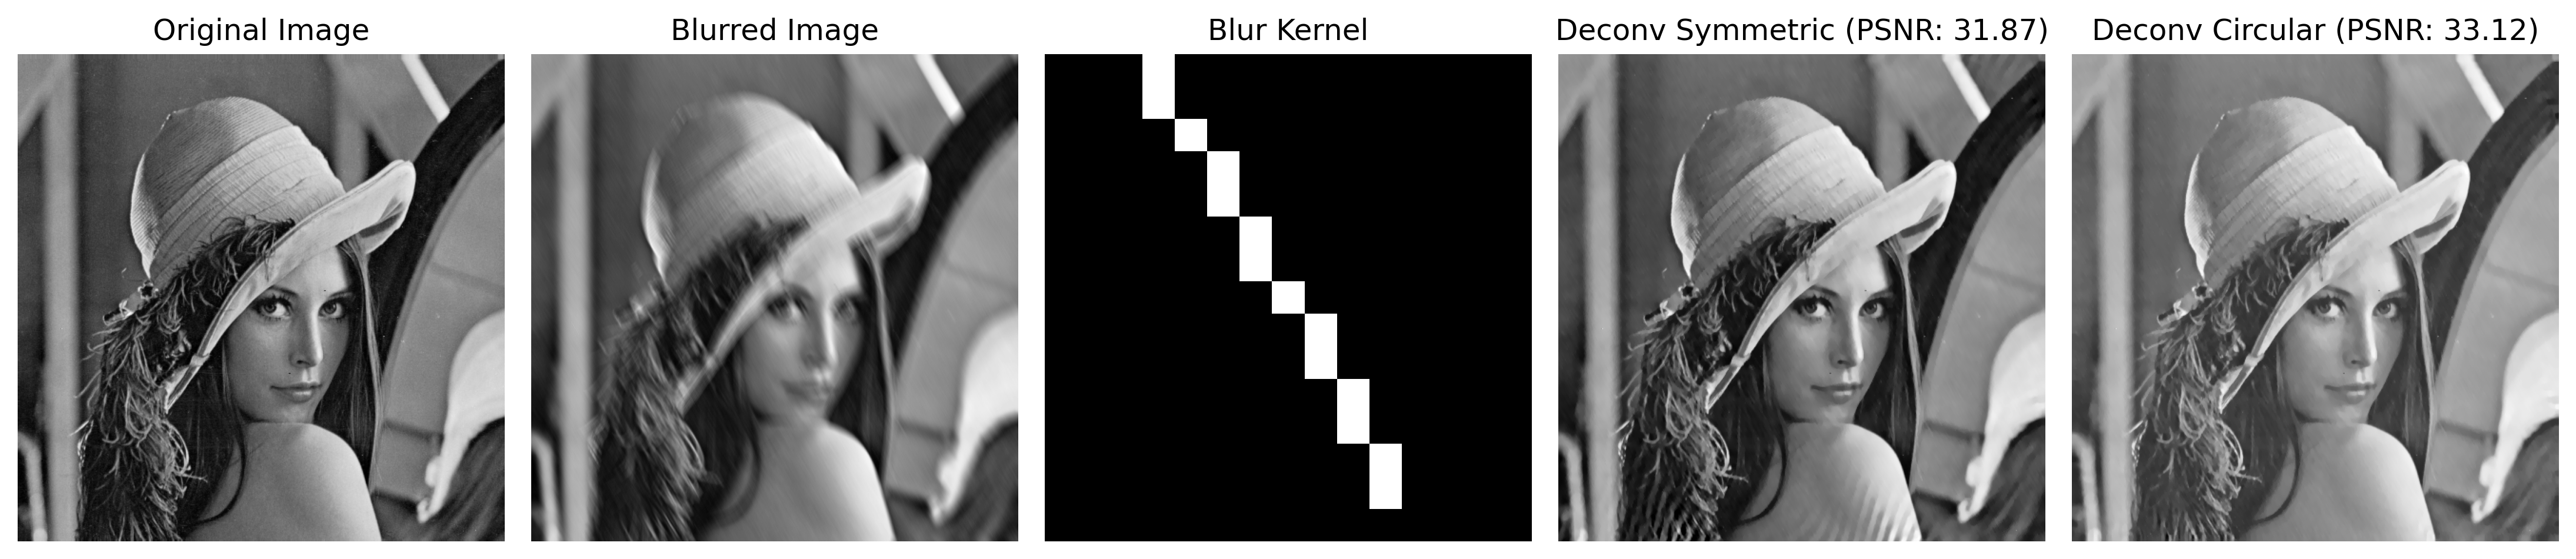
\includegraphics[width=1\linewidth]{../results/circular_vs_symmetric.png}
    \caption{Comparison of deconvolution method with symmetric vs circular boundary conditions.}
    \label{fig:noise_kernel_comparison}
\end{figure}    


\subsection{TV-Deconvolution with known kernel vs estimated kernel}

\begin{figure}[H]
    \centering
    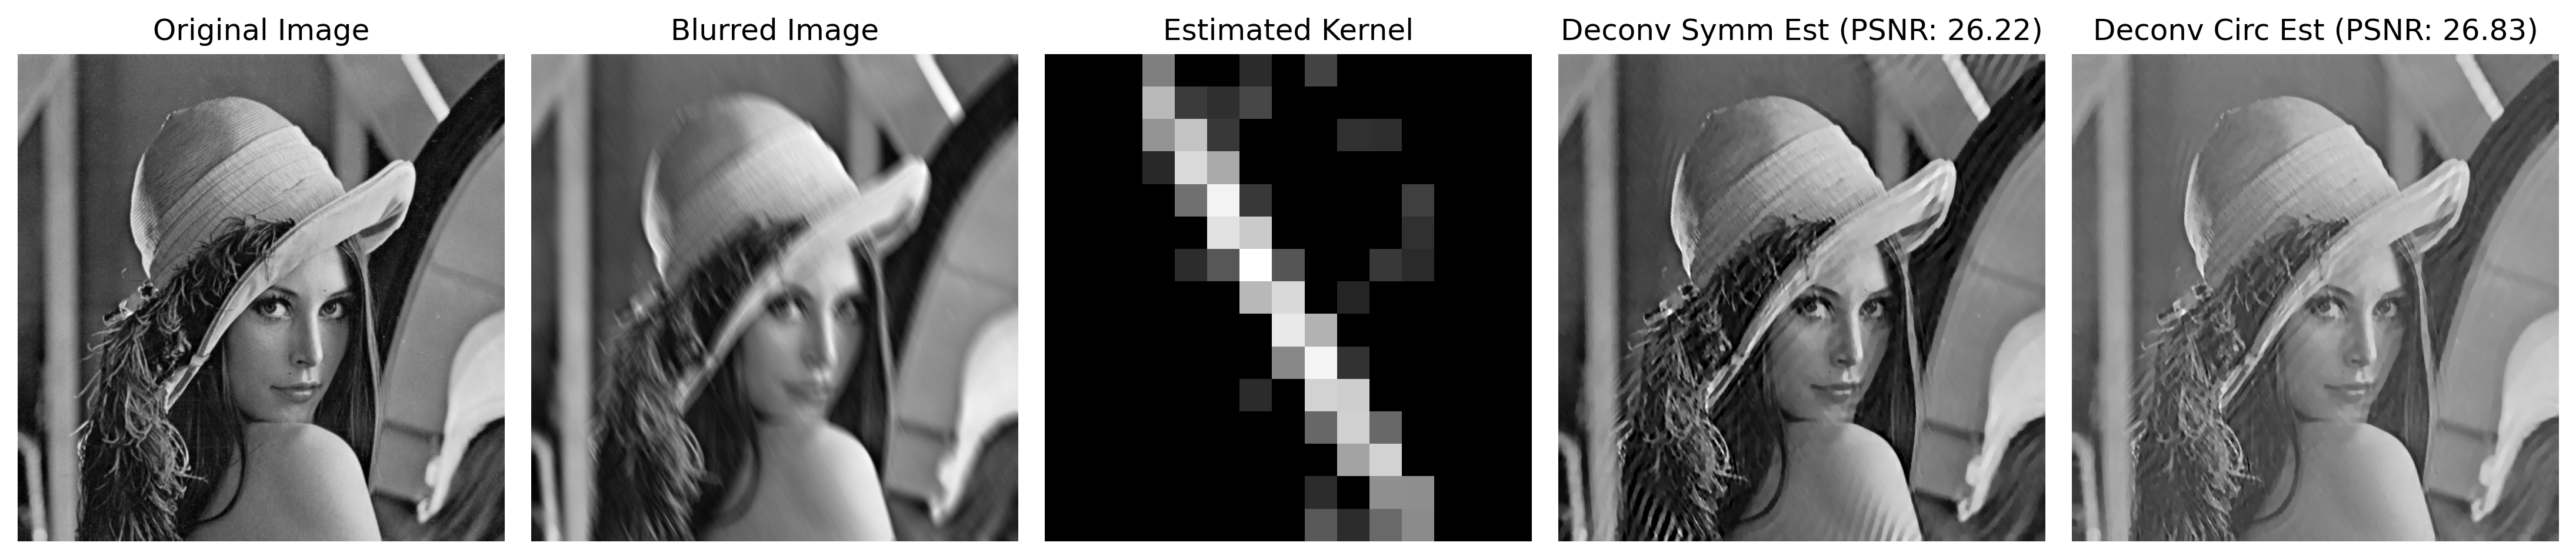
\includegraphics[width=1\linewidth]{../results/circular_vs_symmetric_estimated.png}
    \caption{Comparison of deconvolution with estimated kernel (symmetric vs circular).}
    \label{fig:noise_kernel_comparison}
\end{figure}   


\subsection{TV-Deconvolution robustness to Noise}
\begin{figure}[H]
    \centering
    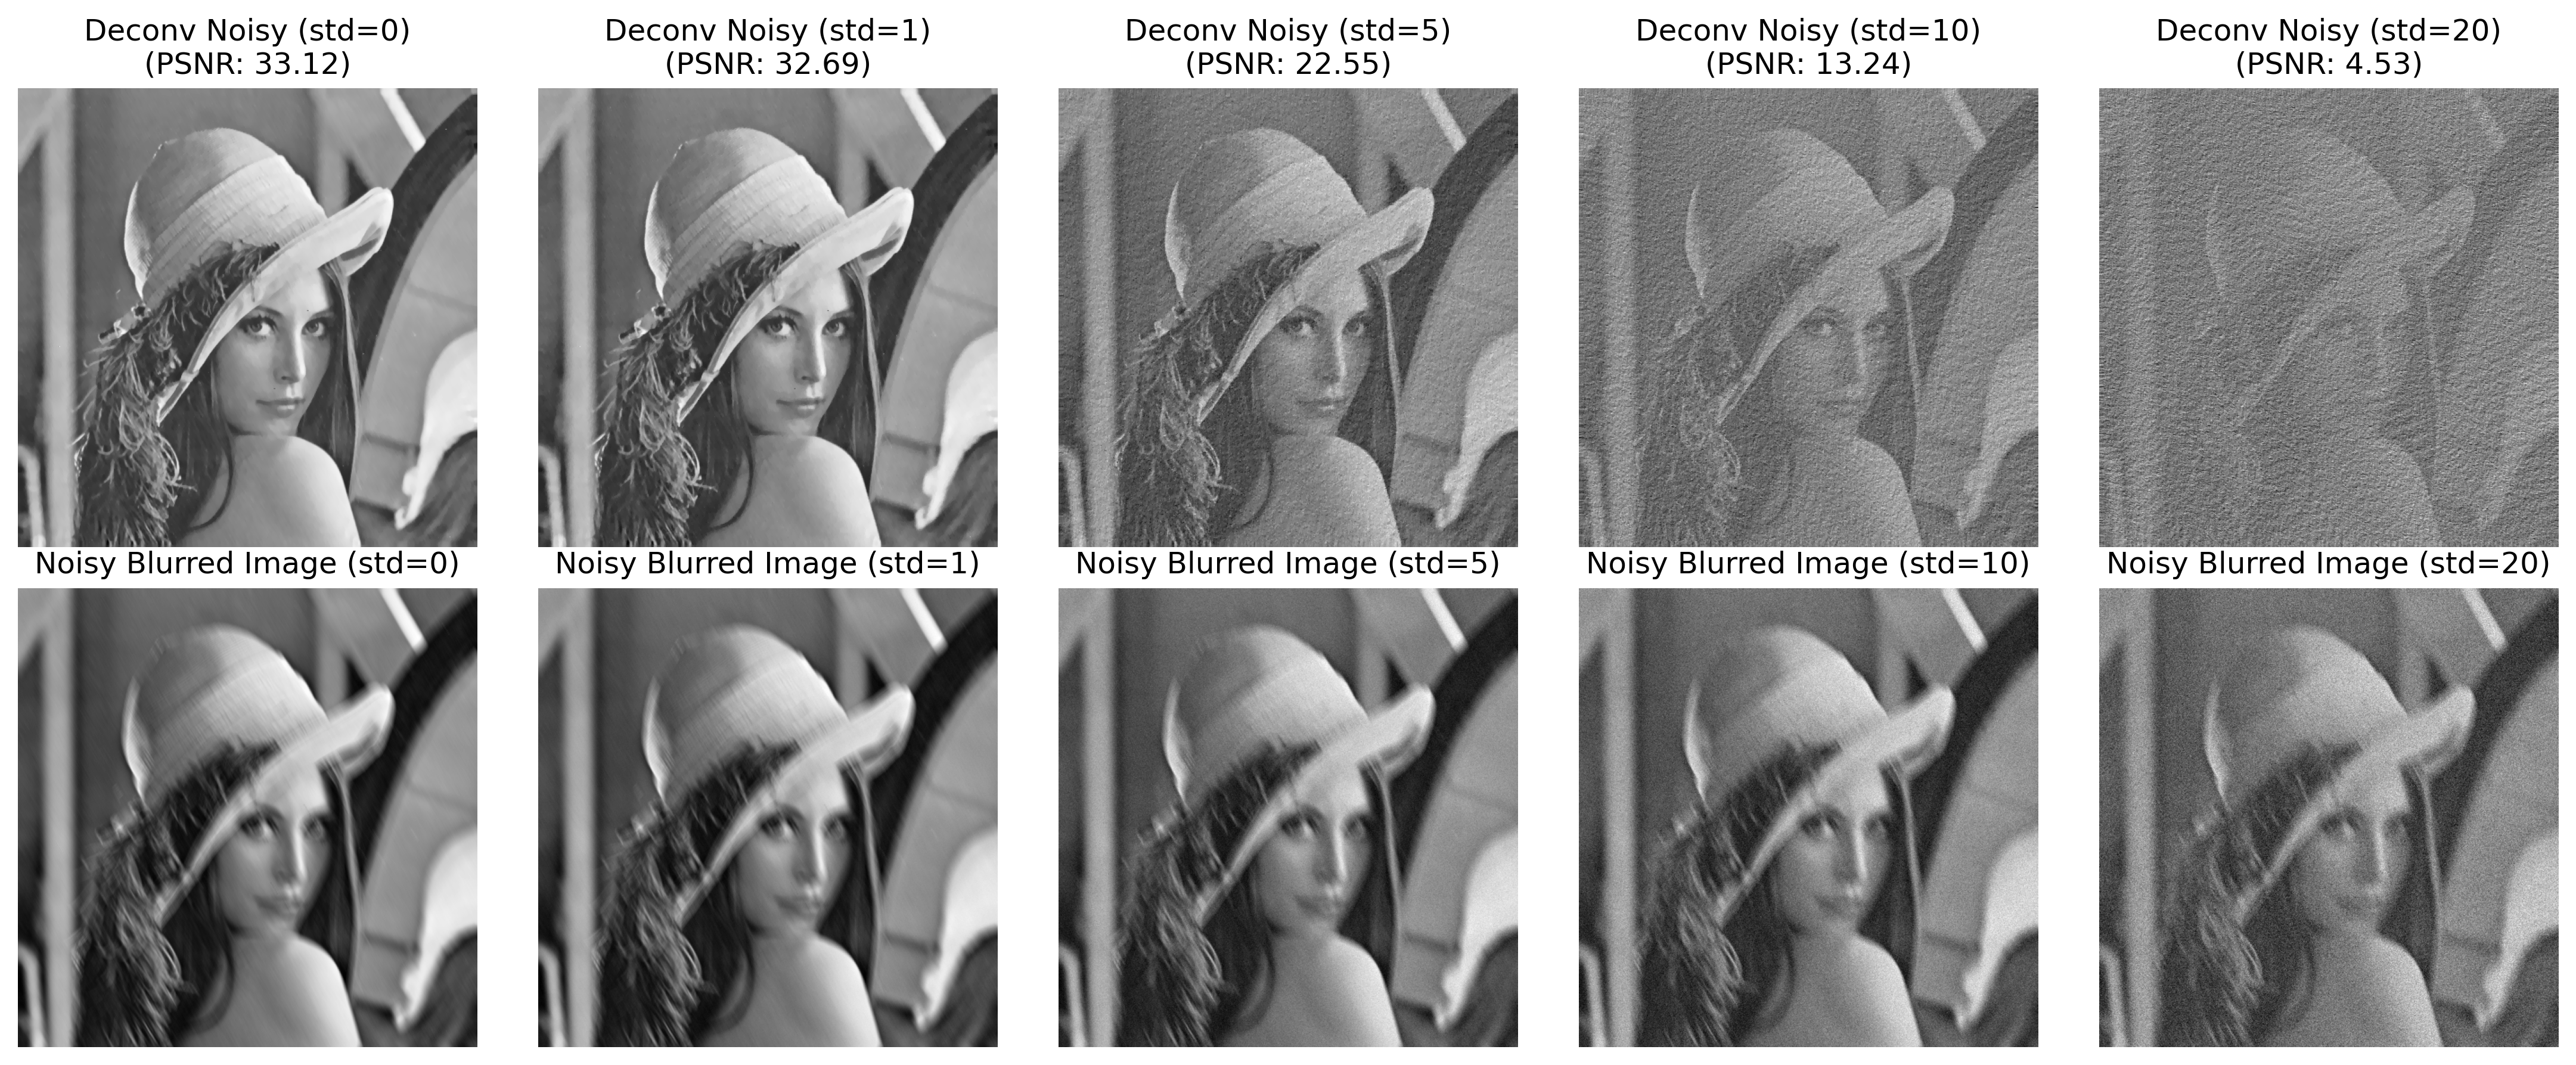
\includegraphics[width=1\linewidth]{../results/tvdeconv_noise_test_circ.png}
\end{figure}

\begin{figure}[H]
    \centering
    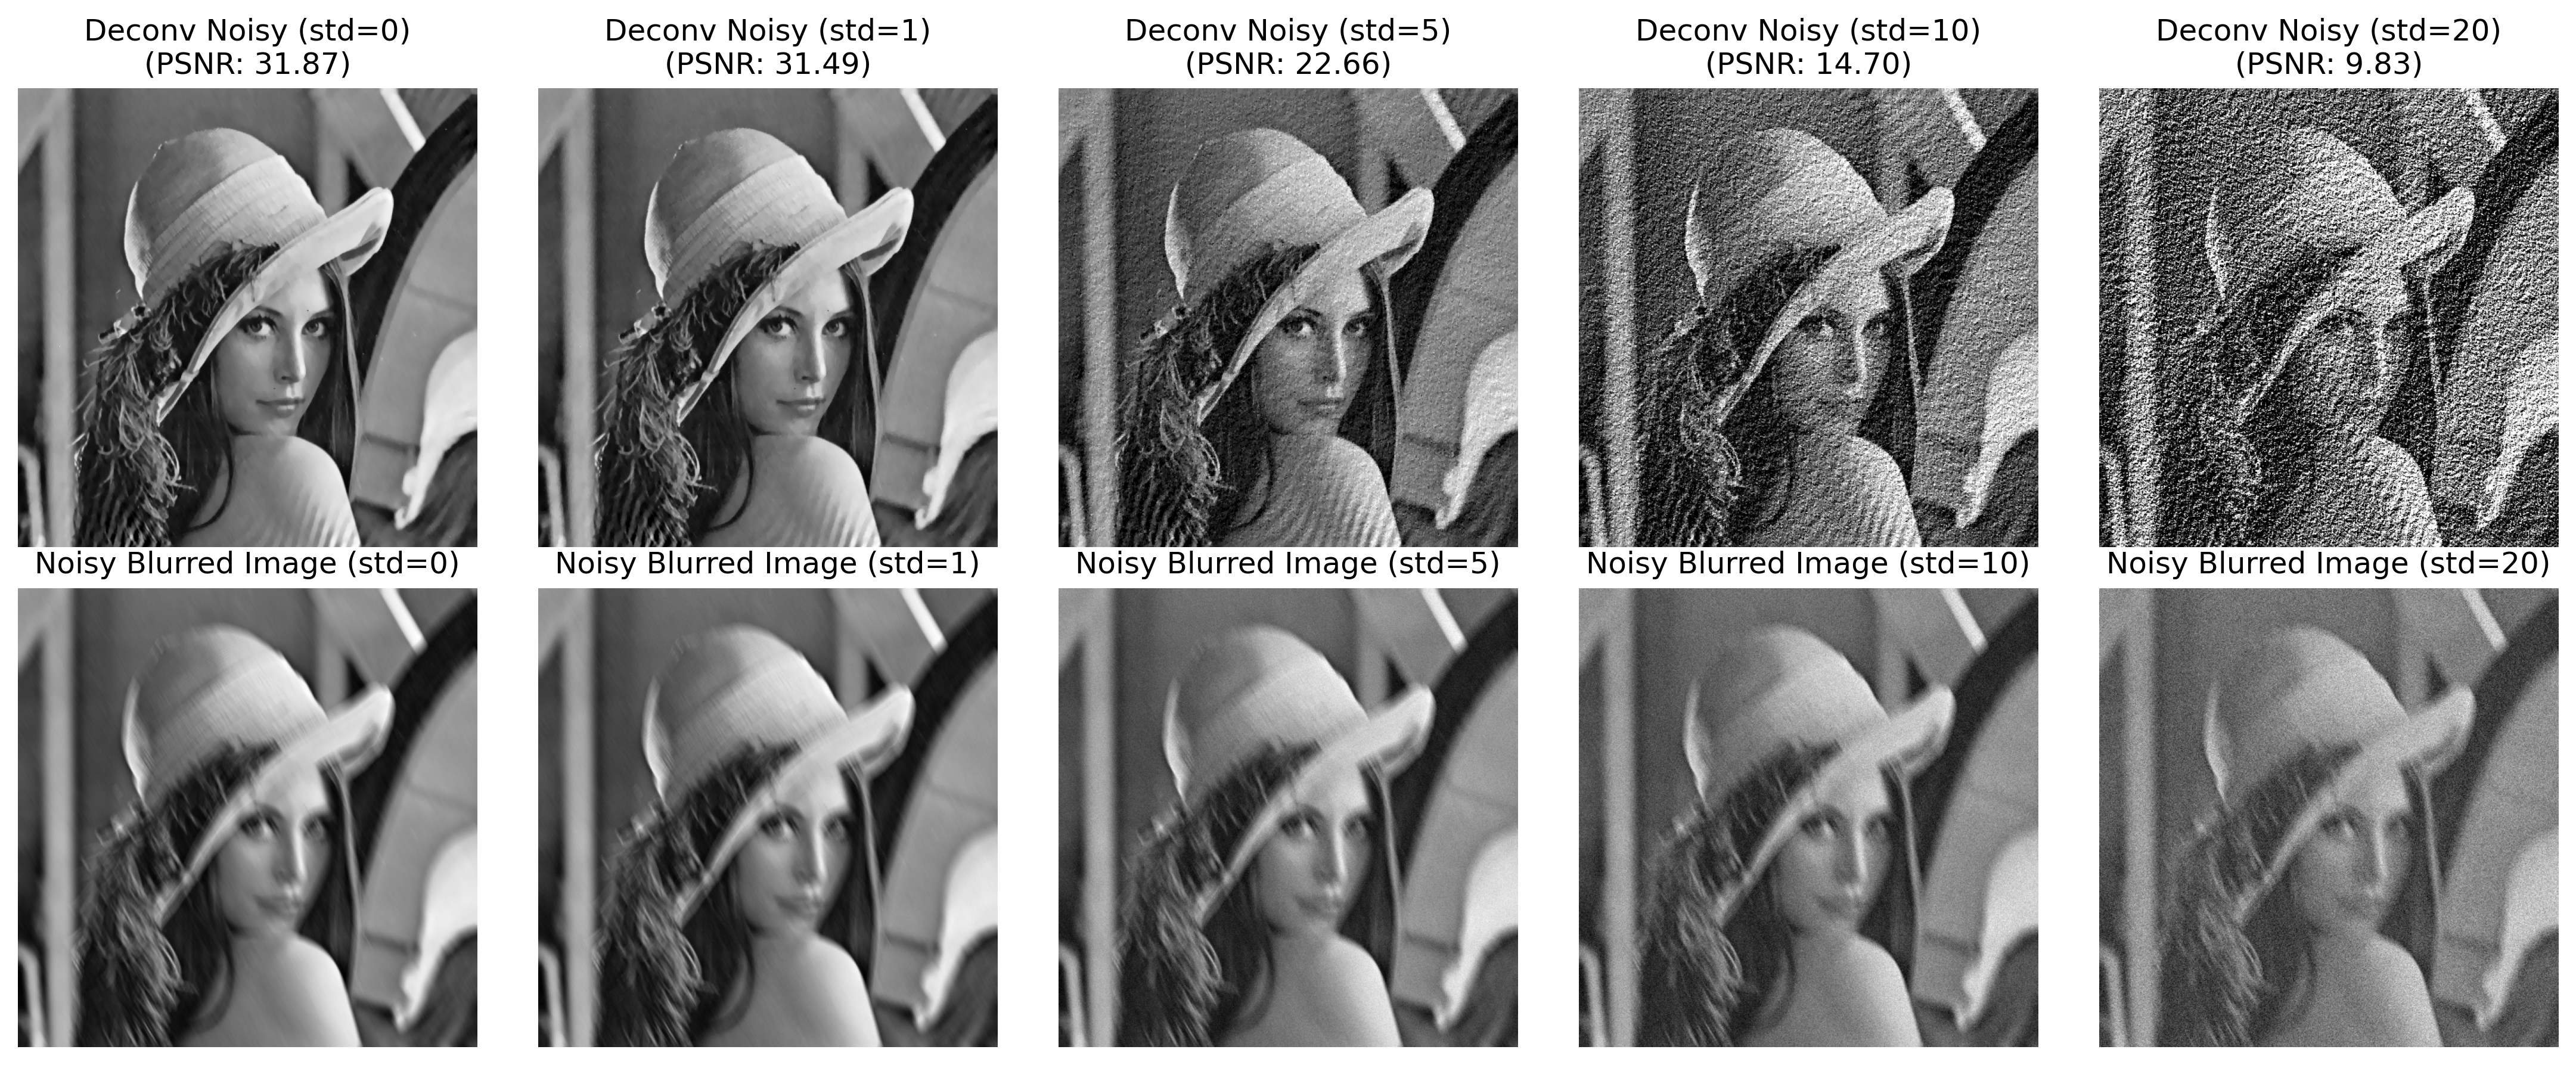
\includegraphics[width=1\linewidth]{../results/tvdeconv_noise_test_symm.png}
    \caption{Comparison of deconvolution robustness to noise with circular and symmetric boundary conditions.}
    \label{fig:noise_kernel_comparison}
\end{figure}

Figure~\ref{fig:noise_kernel_comparison} illustrates the behaviour of the TV--deconvolution
algorithm in the presence of additive impulsive noise for both circular and symmetric
boundary conditions. For low noise levels the reconstruction quality degrades only
slightly: the TV prior is strong enough to suppress a part of the outliers while still
preserving the main edges, so the PSNR remains close to the noise–free case. As the
noise standard deviation increases, however, the $L^2$ data–fidelity term becomes
poorly adapted to the impulsive noise model: a few very large residuals are heavily
penalised and the algorithm tends to fit these peaks instead of rejecting them. After
deconvolution, these sparse outliers are spread by the inverse filter and appear as
structured patterns or textures, which explains the rapid drop in PSNR and the
strong artefacts at high noise levels.

The choice of boundary conditions has a visible impact on the result. With circular
boundary conditions, the convolution operator is modeled as a circulant matrix,
implicitly assuming that the image is periodic. This allows a very efficient solution
in the Fourier domain, but it also couples opposite borders of the image: noise and
ringing artefacts are wrapped around and re–injected everywhere in the field of view.
When the noise becomes large, the TV regularisation then drives the solution towards
an almost piecewise–constant image with a ``greyish'' appearance, which strongly
reduces the PSNR. Symmetric boundary conditions, on the other hand, correspond to an
even extension of the image outside the domain. This avoids wrap–around artefacts
and yields reconstructions that are sharper and visually more faithful in the central
region, which explains the systematically higher PSNR. However, the mirroring of
structures at the border interacts with the inverse filter and the TV prior, so that
spurious oscillations and edge artefacts may appear near the image boundaries despite
the overall gain in visual quality.



\subsection{Hyperparameters tuning for TV-Deconvolution}

\begin{figure}[H]
    \centering
    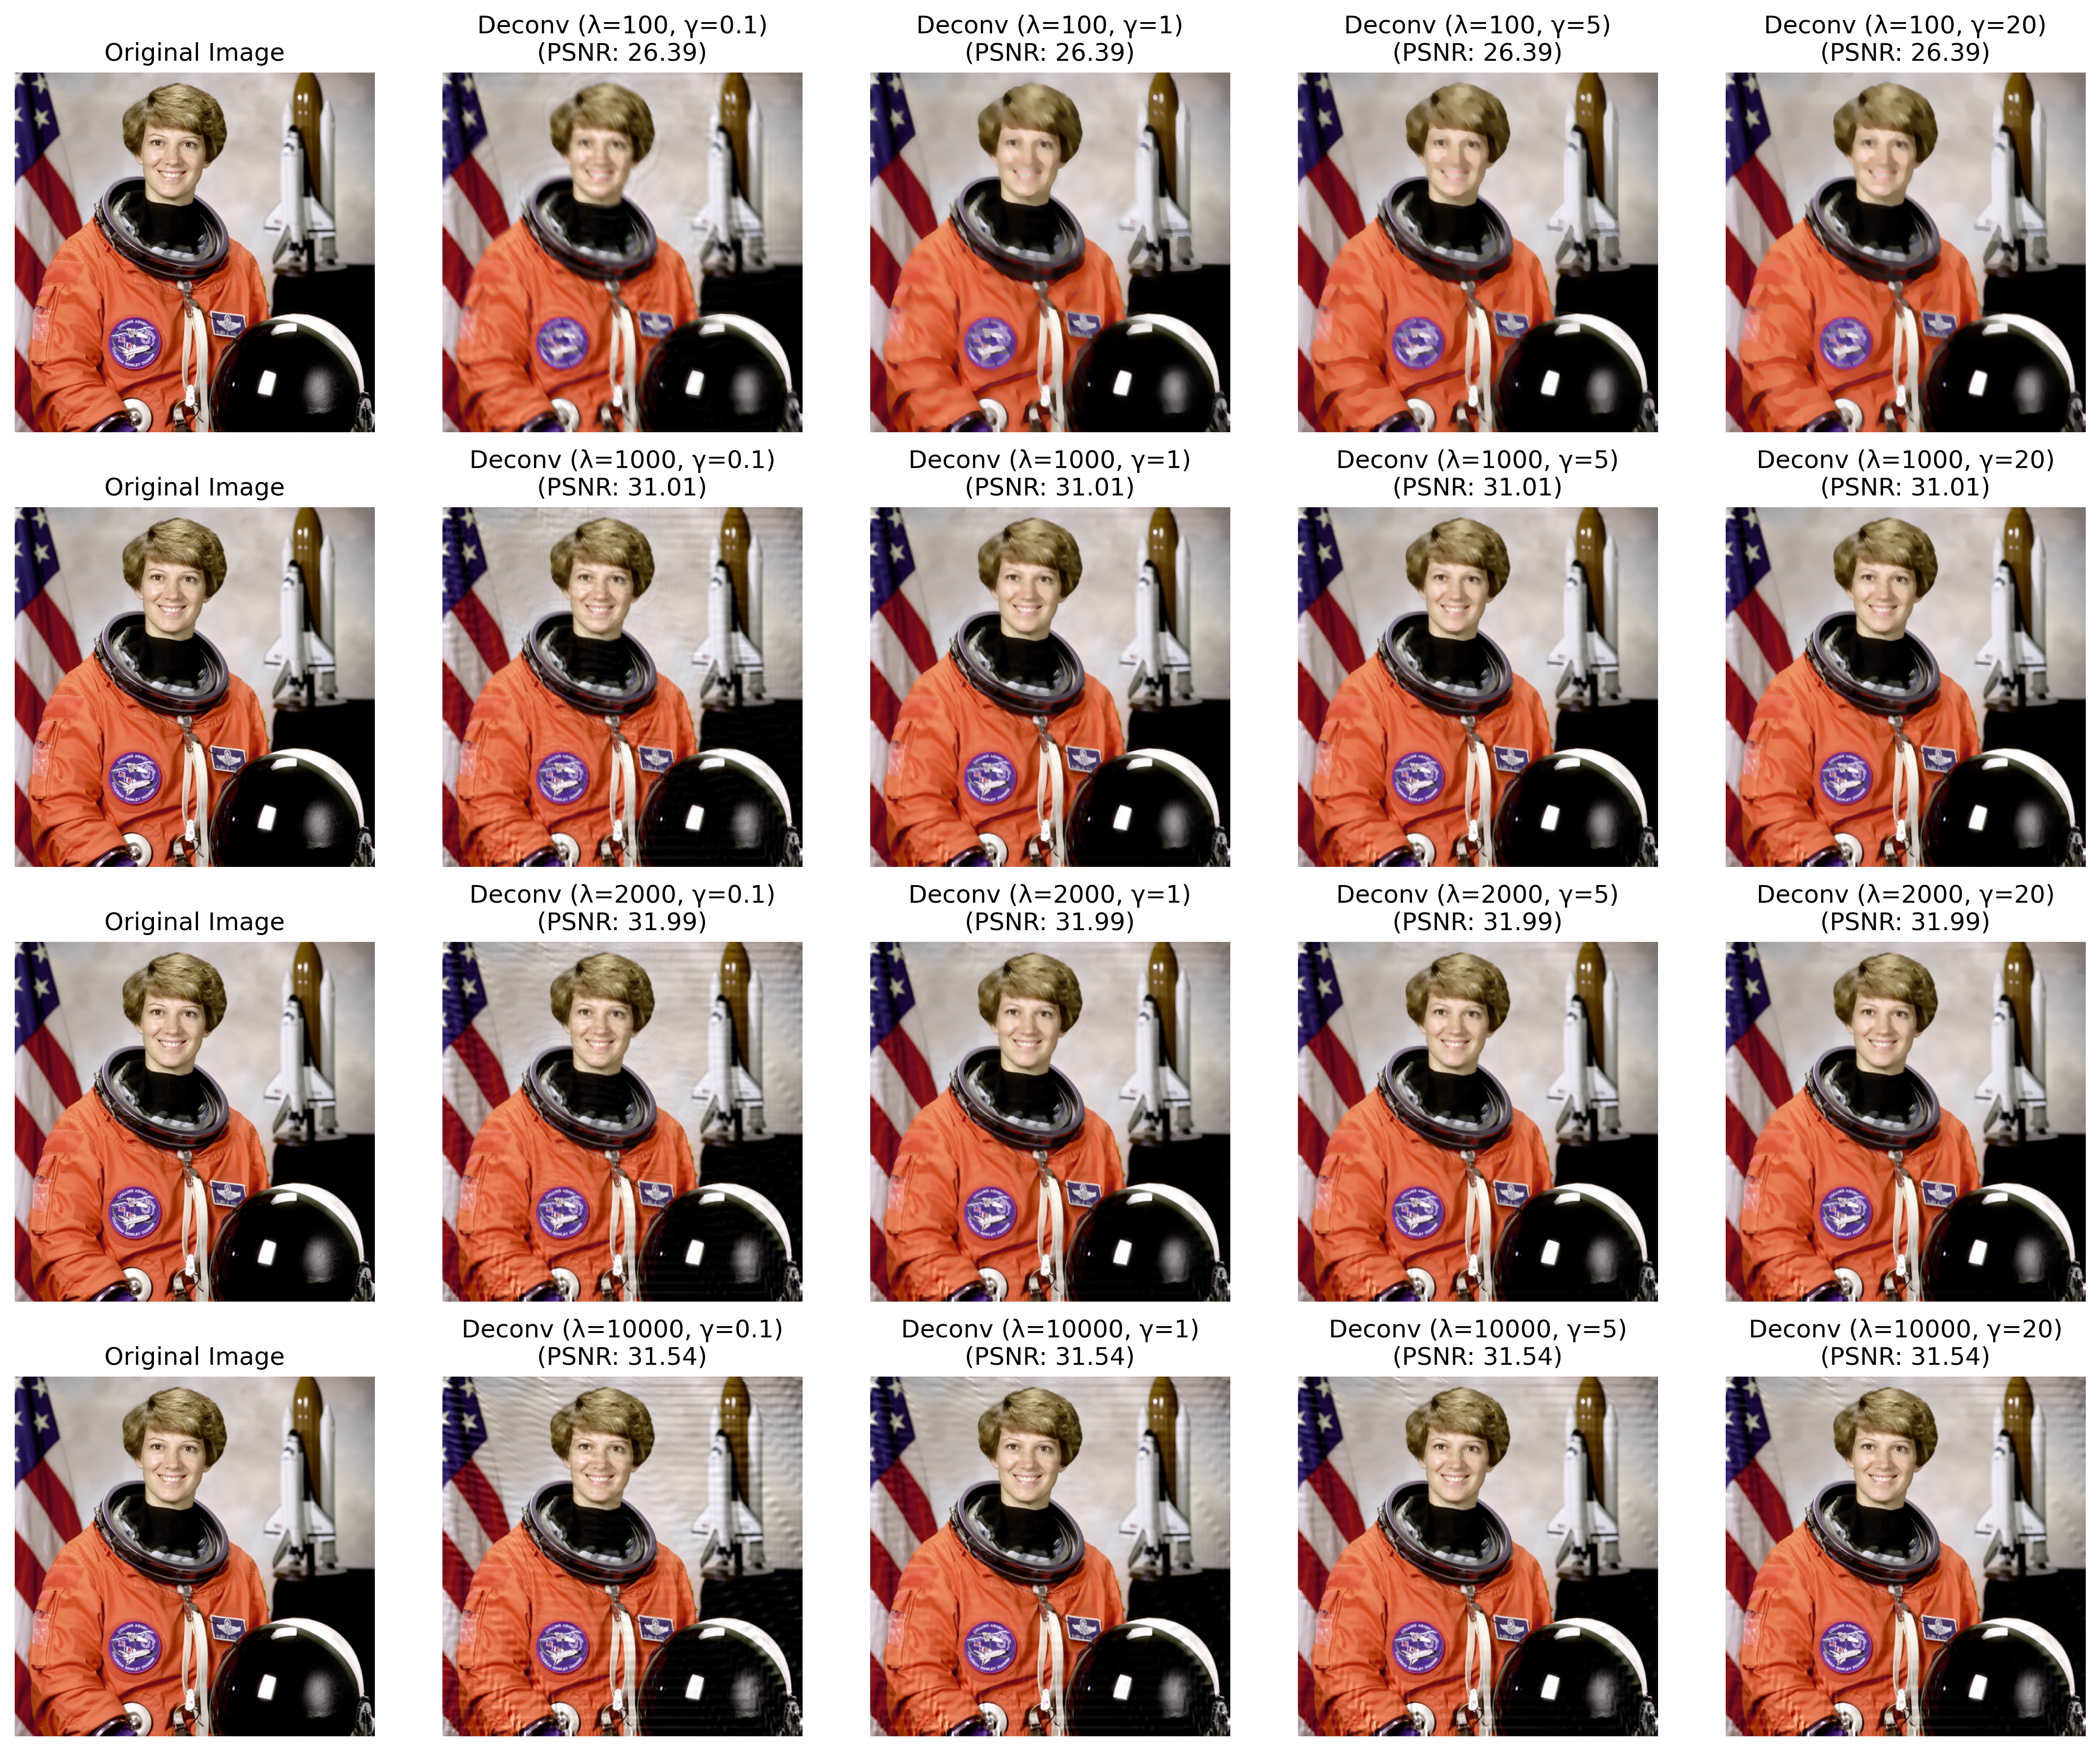
\includegraphics[width=1\linewidth]{../results/hyperparam_test_circ.png}
    \caption{Tuning of hyperparameters $(\lambda,\gamma)$ for TV-deconvolution.}
    \label{fig:noise_kernel_comparison}
\end{figure}

\begin{figure}[H]
    \centering
    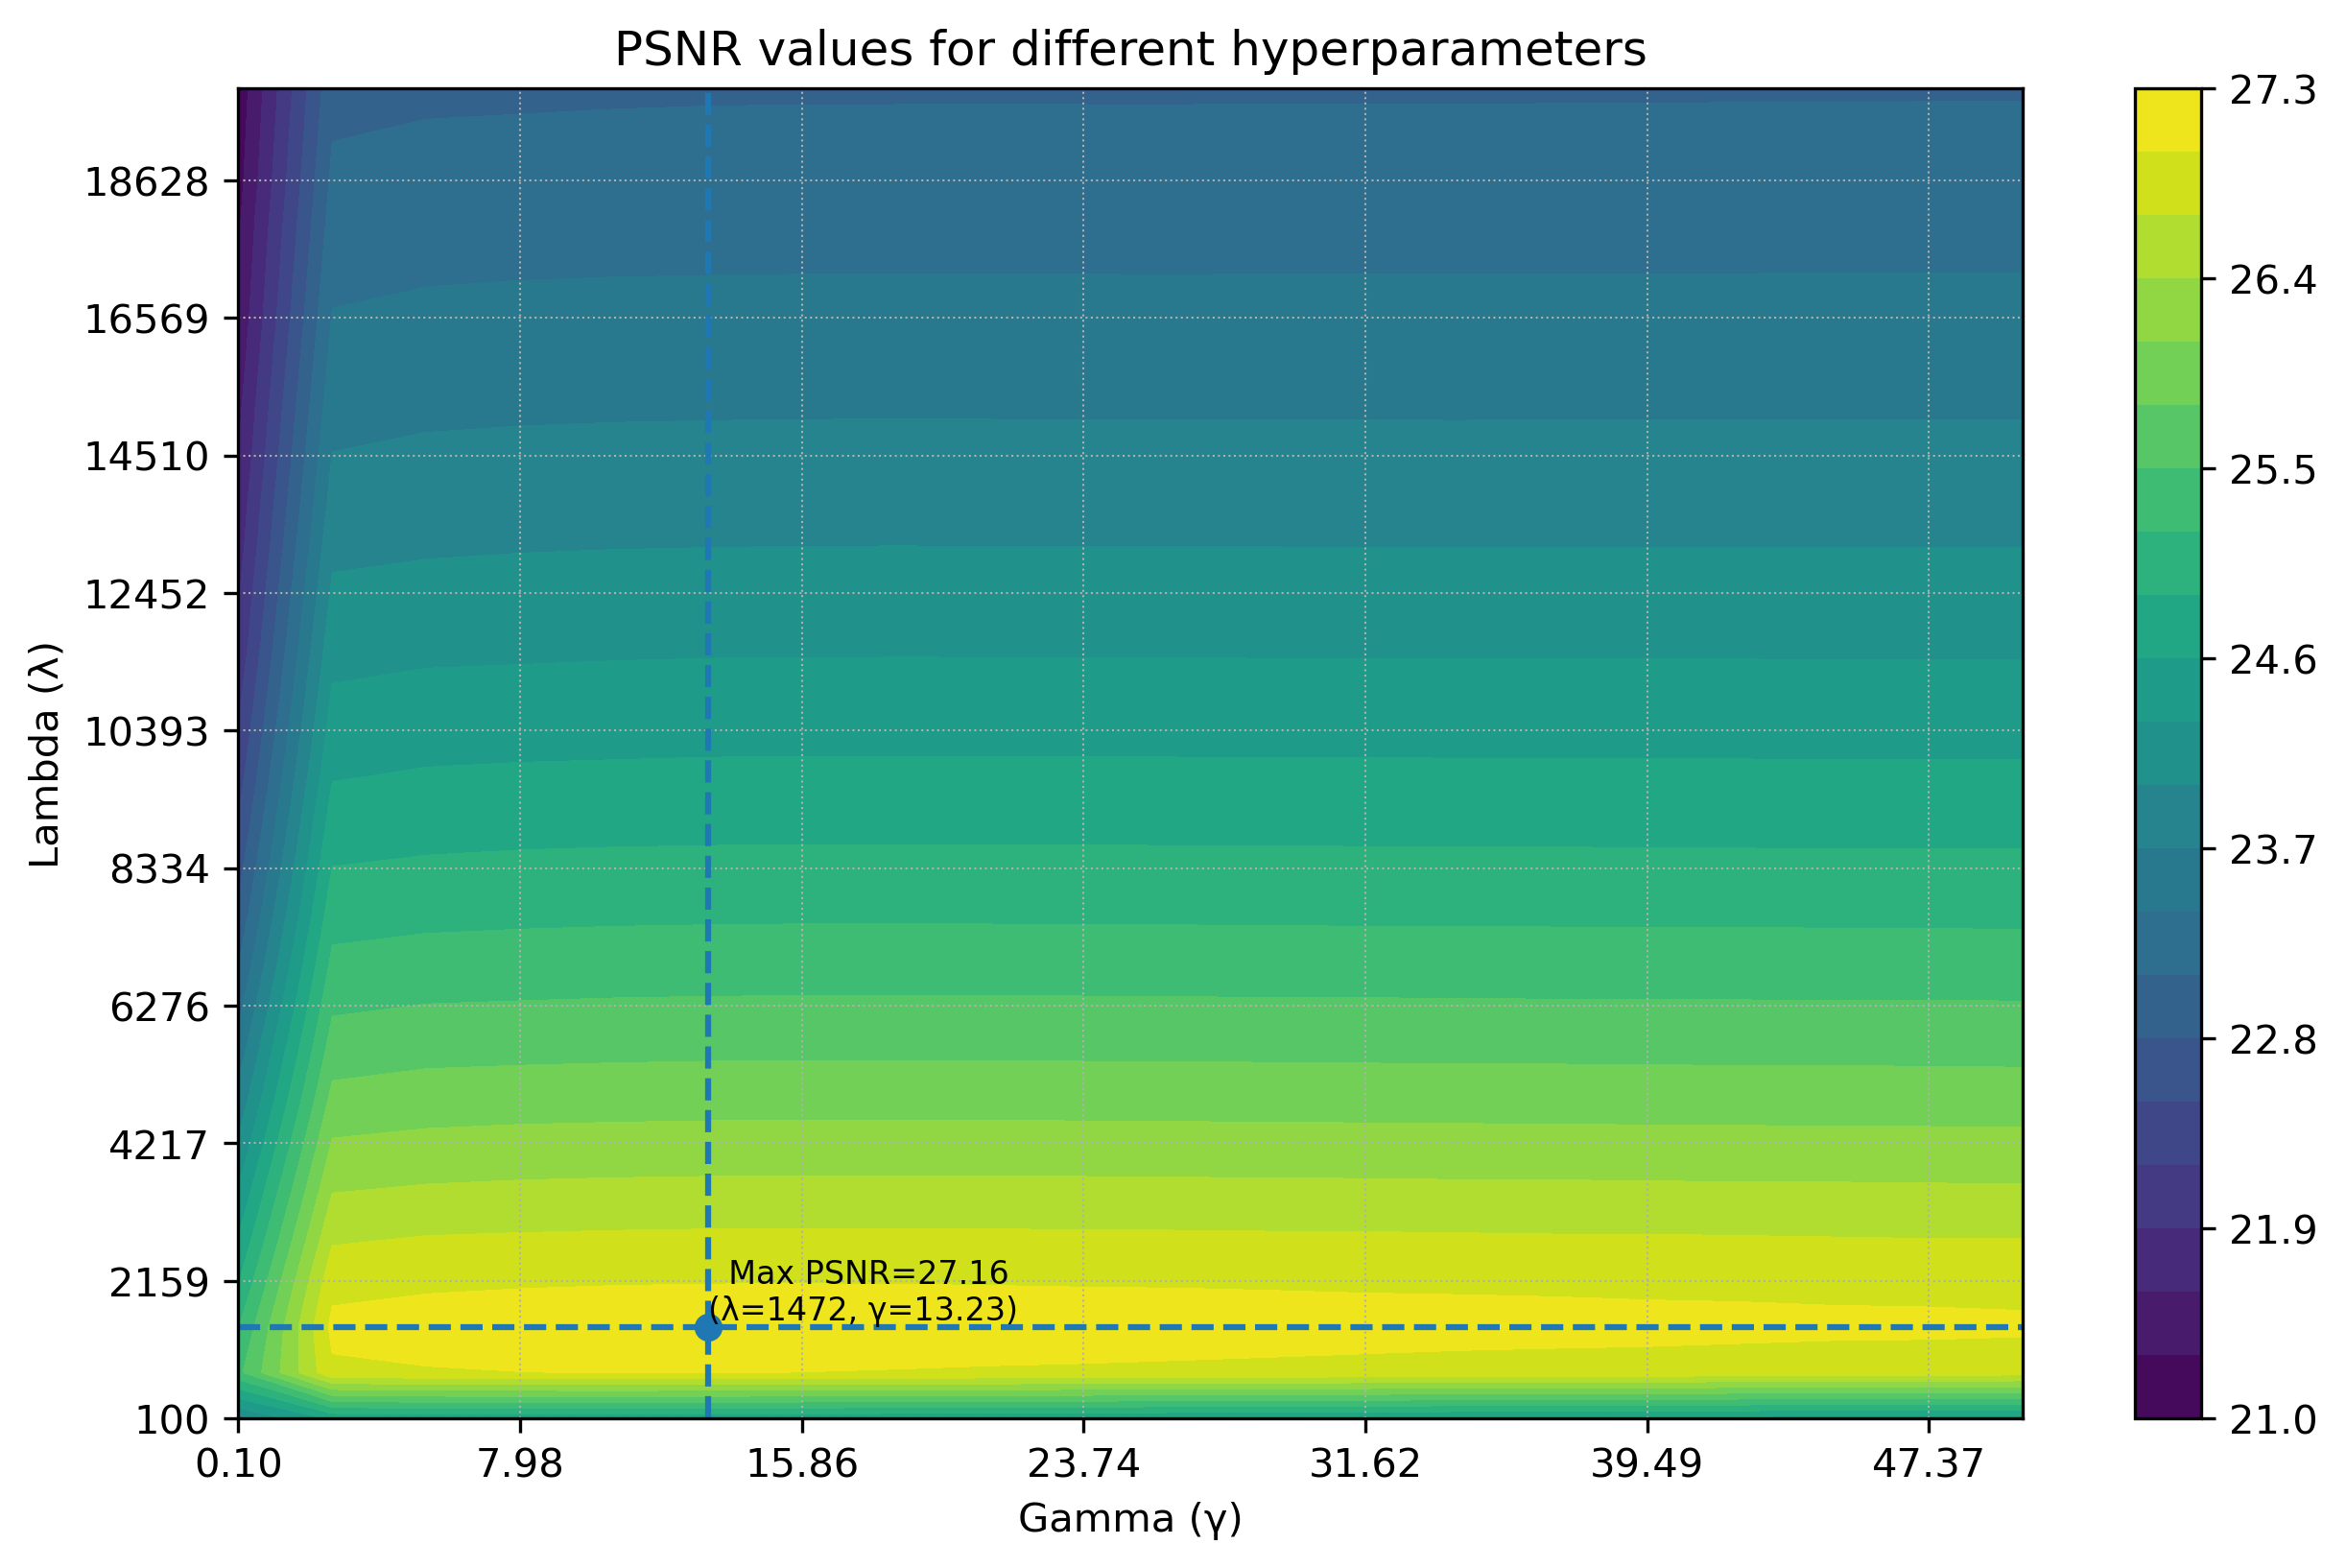
\includegraphics[width=0.8\linewidth]{../results/hyperparameter_tuning.png}
    \caption{PSNR heatmap for different hyperparameters $(\lambda,\gamma)$ for TV-deconvolution.}
    \label{fig:noise_kernel_comparison}
\end{figure}

Figure~\ref{fig:noise_kernel_comparison} (right) shows a PSNR heatmap as a function of the two TV--deconvolution hyperparameters $(\lambda,\gamma)$. The regularisation weight $\lambda$ controls the trade--off between data fidelity and TV smoothing, while $\gamma$ is the penalty parameter that enforces the constraint $d = \nabla u$ in the split--Bregman scheme. 
For very small values of $\lambda$, the reconstruction is clearly under--regularised: the image remains noticeably blurred and may still contain ringing artefacts, which results in a low PSNR. 
As $\lambda$ increases, the image becomes sharper and the PSNR quickly improves, reaching a maximum of about $\mathrm{PSNR} = 27.2\,\mathrm{dB}$ around $(\lambda^\star, \gamma^\star) \simeq (1472, 13.2)$. 
Beyond this region, larger $\lambda$ values start to over--smooth the solution: edges are still preserved but fine textures and low--contrast details are progressively attenuated, which decreases the PSNR. 
The behaviour with respect to $\gamma$ is less critical: there exists a broad plateau of good performance for intermediate values, whereas too small or too large $\gamma$ slightly degrades the restoration, mainly by slowing down or destabilising the split--Bregman iterations. Overall, the map indicates that the method is reasonably robust to the choice of $\gamma$, but more sensitive to the regularisation weight $\lambda$.


\subsection{Kernel estimation Robustness to Noise}

In what precedes, we assumed $v = h*u$ to have the estimation of $|\hat{h}(\xi_\theta)|^2$. If we add an impulse noise $b$, obtain : 
$$\mathcal{F}(R(D_{\theta}(v+b)))(\xi_\theta) = \|\bm{\xi}_\theta\|^2 (|\hat{h}(\bm{\xi}_\theta)|^2|\hat{u}(\bm{\xi}_\theta)|^2 + |\hat{b}(\bm{\xi}_\theta)|^2)$$
So the noise will add a bias to the estimation of $|\hat{h}|$, especially on high frequencies which will wider the autocorrelation and wrong the estimation.\\

\begin{figure}[H]
    \centering
    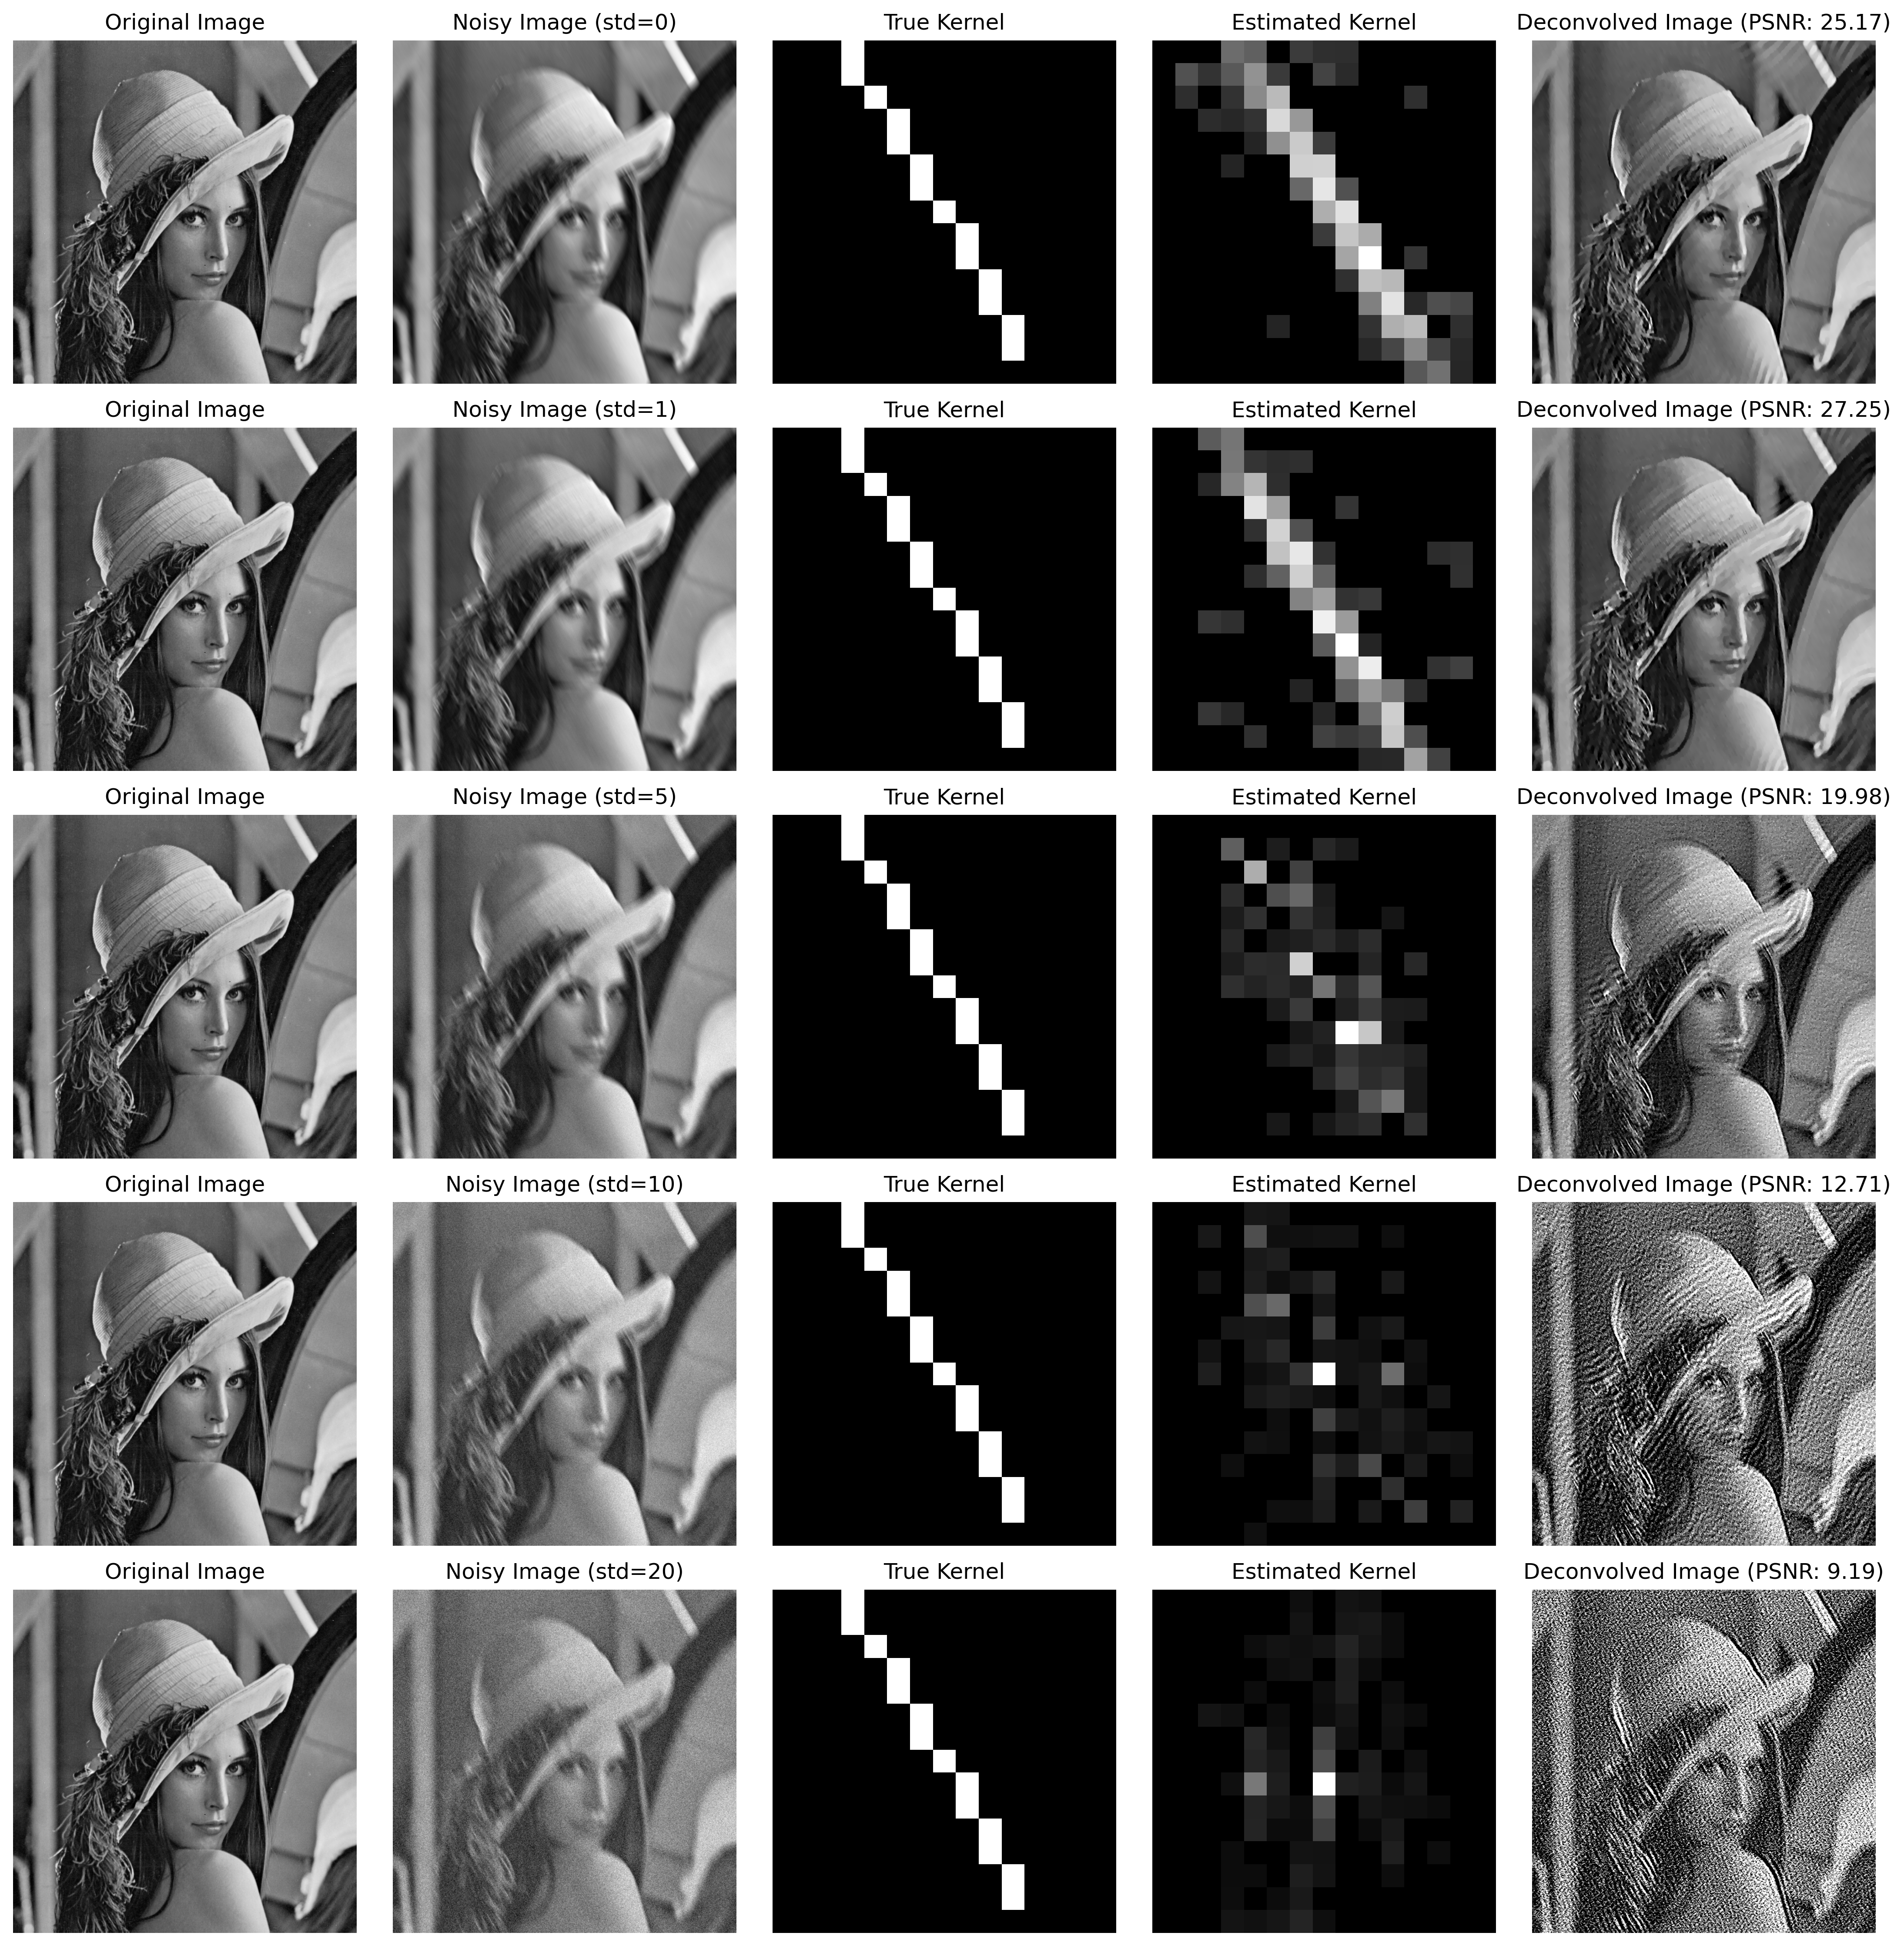
\includegraphics[width=1\linewidth]{../results/noise_test.png}
    \caption{Comparison of estimated kernels with different noise levels (SNR in dB).}
    \label{fig:noise_kernel_comparison}
\end{figure}  

Figure~\ref{fig:noise_kernel_comparison} illustrates more precisely how the Goldstein--Fattal
kernel estimation behaves in the presence of additive noise. For noise-free or mildly noisy
observations ($\mathrm{std}=0$ and $\mathrm{std}=1$), the estimated kernel remains close to the
ground-truth diagonal motion blur and the subsequent TV deconvolution reaches PSNR values
around $25$--$27\,\mathrm{dB}$. This is consistent with the theoretical model: after whitening,
the spectrum of a sharp image should be approximately flat, so the residual spectral
irregularities mainly encode the blur kernel. When the noise level increases
($\mathrm{std}\geq 5$), the whitening step amplifies the high-frequency noise and the 1D
autocorrelations used to recover $|\hat h|^2$ become strongly corrupted; as a result, the
estimated kernels lose their elongated structure and concentrate most of their energy on a few
spurious peaks. The deconvolved images then exhibit heavy ringing and texture-like artefacts,
and the PSNR drops dramatically (down to about $9\,\mathrm{dB}$ for $\mathrm{std}=20$). These
experiments confirm the analysis of Anger \emph{et al.}, namely that the Goldstein--Fattal
estimator is reasonably stable for low noise levels but degrades quickly when the noise variance
becomes too large, since the projection-based whitening does not intrinsically denoise the
observations and mainly transfers the noise into the estimated kernel.%


\subsection{Kernel size robustness}

\begin{figure}[H]
    \centering
    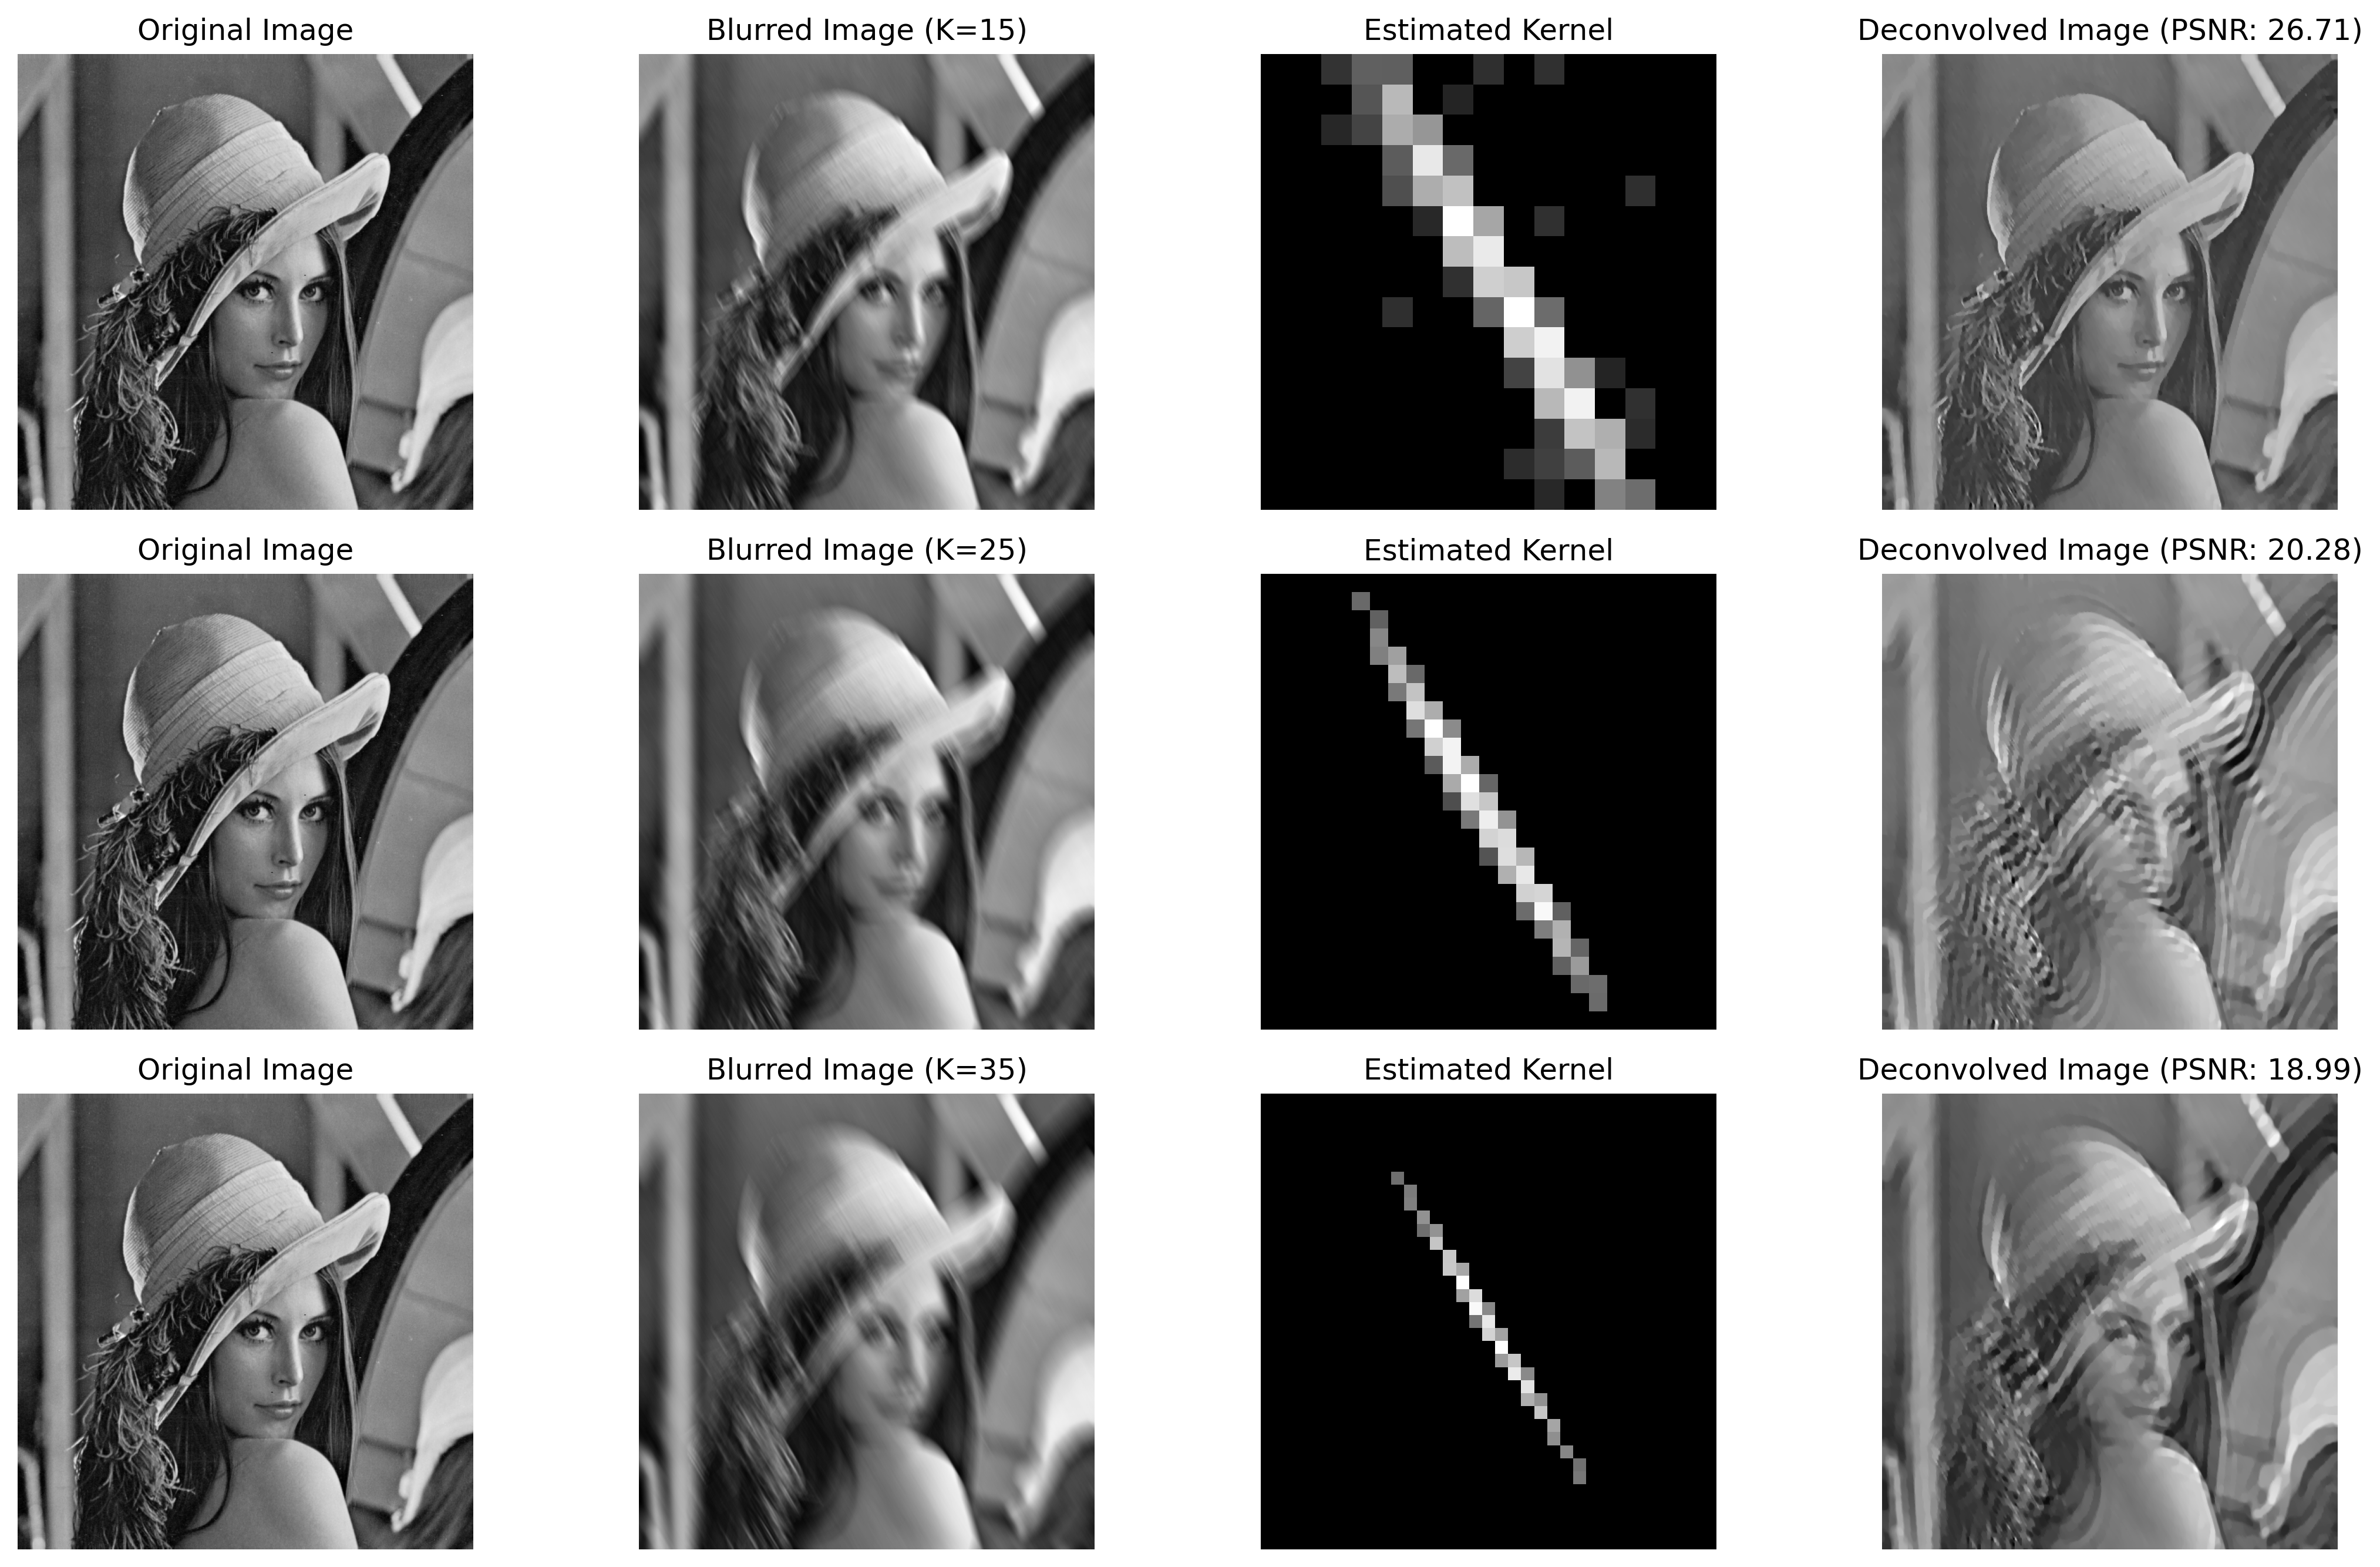
\includegraphics[width=1\linewidth]{../results/kernel_size_test_circ.png}
    \caption{Comparison of estimated kernels and deconvolved images for different kernel sizes
    ($K=15$, $K=25$, $K=35$).}
    \label{fig:kernel_size_robustness}
\end{figure}


Figure~\ref{fig:kernel_size_robustness} illustrates the influence of the blur-kernel size on the
Goldstein--Fattal estimation procedure and on the subsequent TV deconvolution. For a moderate
motion length ($K=15$), the estimated kernel is reasonably close to the true diagonal blur and
the restored image remains visually sharp, with a PSNR of about $26.7\,\mathrm{dB}$. As the
kernel size increases ($K=25$ and $K=35$), the degradation becomes much more pronounced: although
the estimated kernels still exhibit an elongated diagonal structure, they contain many secondary
lobes and their support no longer matches the true one. The corresponding deconvolved images are
dominated by strong oscillations and wavy artefacts along the blur direction, and the PSNR drops
to roughly $20.3\,\mathrm{dB}$ and $19.0\,\mathrm{dB}$, respectively. This behaviour can be
explained by the fact that long motion blurs remove a large portion of the high–frequency content
of the image, so that the 1D autocorrelations used to estimate $|\hat h|^2$ become increasingly
ill-conditioned and very sensitive to modelling errors. Any mismatch in the recovered support is
then strongly amplified by the inverse filter in the TV–deconvolution step, especially with
circular boundary conditions, which leads to the observed ringing artefacts. Overall, the method
appears reliable for small to moderate kernel sizes, but its performance quickly degrades as the
blur extent grows.

\subsection{Real images test}
\begin{figure}[H]
    \centering
    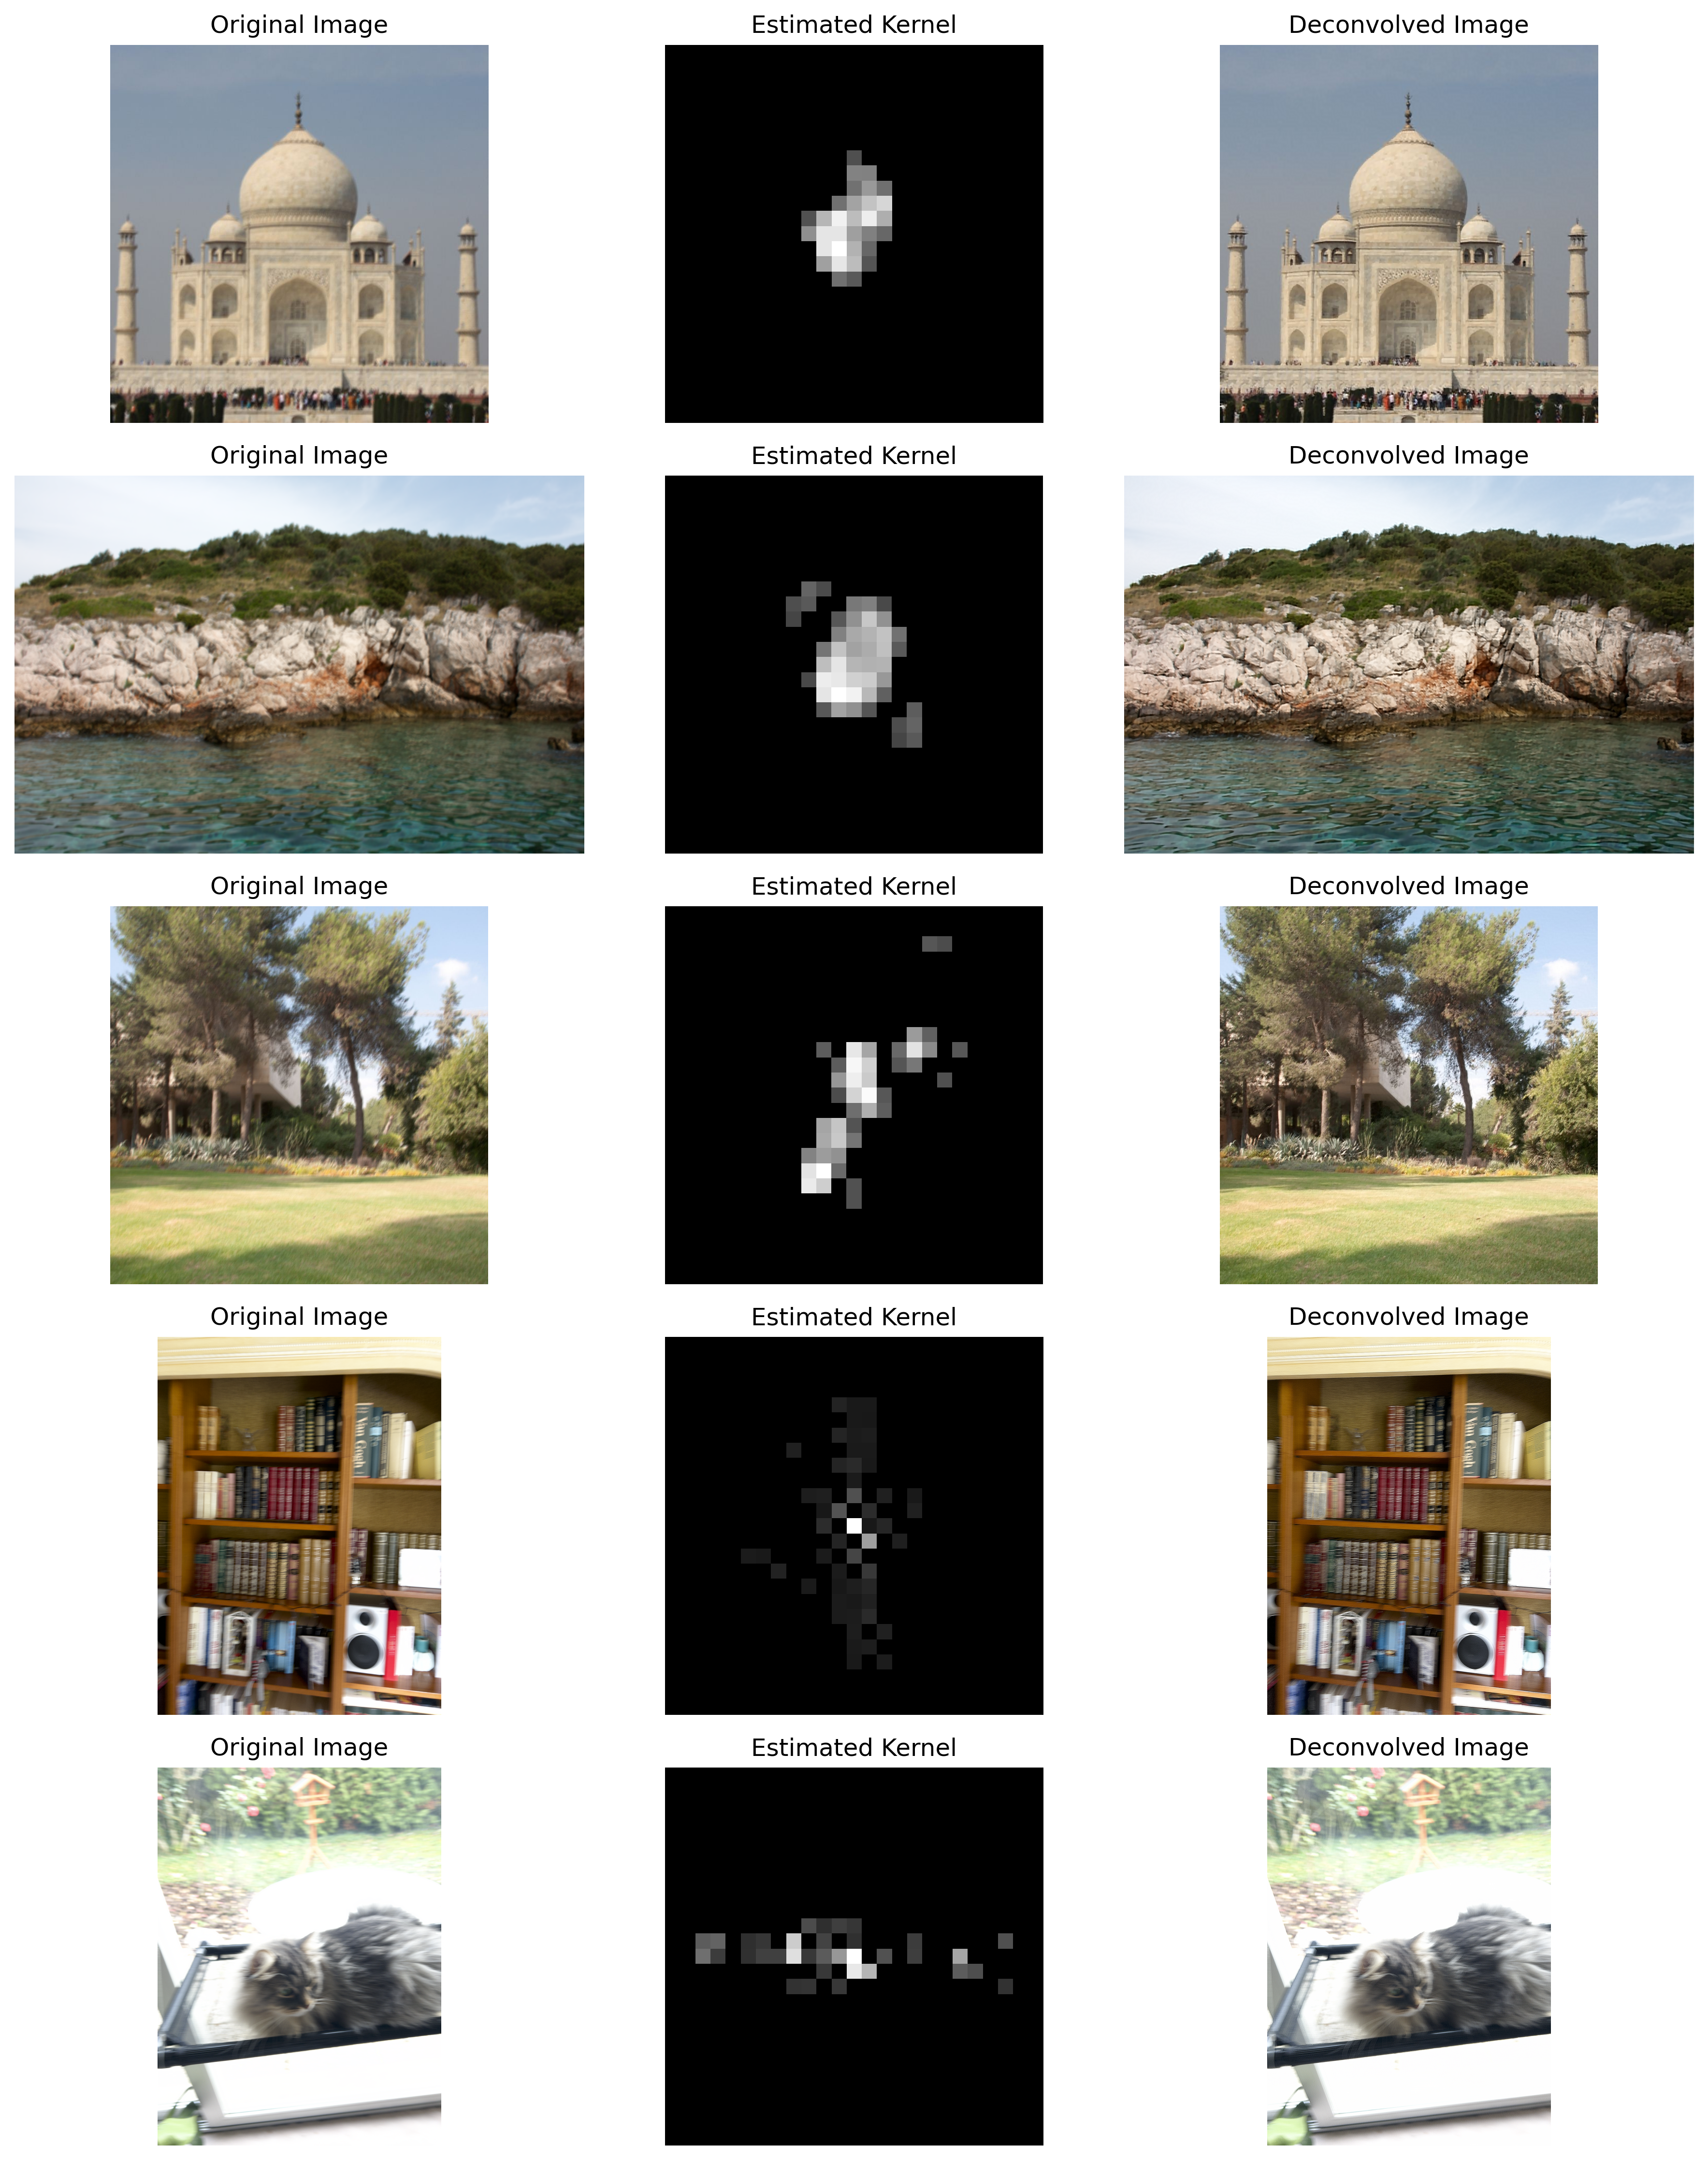
\includegraphics[width=1\linewidth]{../results/real_images_test.png}
    \caption{Comparison of estimated kernels with different noise levels (SNR in dB).}
    \label{fig:noise_kernel_comparison}
\end{figure}

Figure~\ref{fig:noise_kernel_comparison} shows the behaviour of the method on real camera-blurred images. In the first three examples, taken from standard natural-image datasets, the blur remains relatively mild and can be reasonably approximated by a spatially invariant motion kernel. Under these conditions, the Goldstein–Fattal estimator produces compact and coherent kernels with a clear dominant direction, and the subsequent TV deconvolution successfully sharpens the images, restoring edges and fine structures without introducing strong artefacts.

The last two rows, however, correspond to personal RAW photographs captured hand-held, and the method fails to recover meaningful kernels. Here, the camera motion is likely much more complex—combining small 3D rotations, slight lens defocus, sensor noise, and potentially rolling-shutter distortions. Such blur is no longer well modelled by a single convolution kernel. As a result, the estimated kernels become highly fragmented and irregular, and the deconvolution step is unable to restore the images, yielding outputs that remain blurry or exhibit additional artefacts.

These experiments highlight an important limitation: the method performs reliably when the blur is simple and approximately convolutional, but breaks down on realistic handheld RAW images where the true camera motion deviates significantly from the simplified model.

\subsection{Compressed images robustness}

\begin{figure}[H]
    \centering
    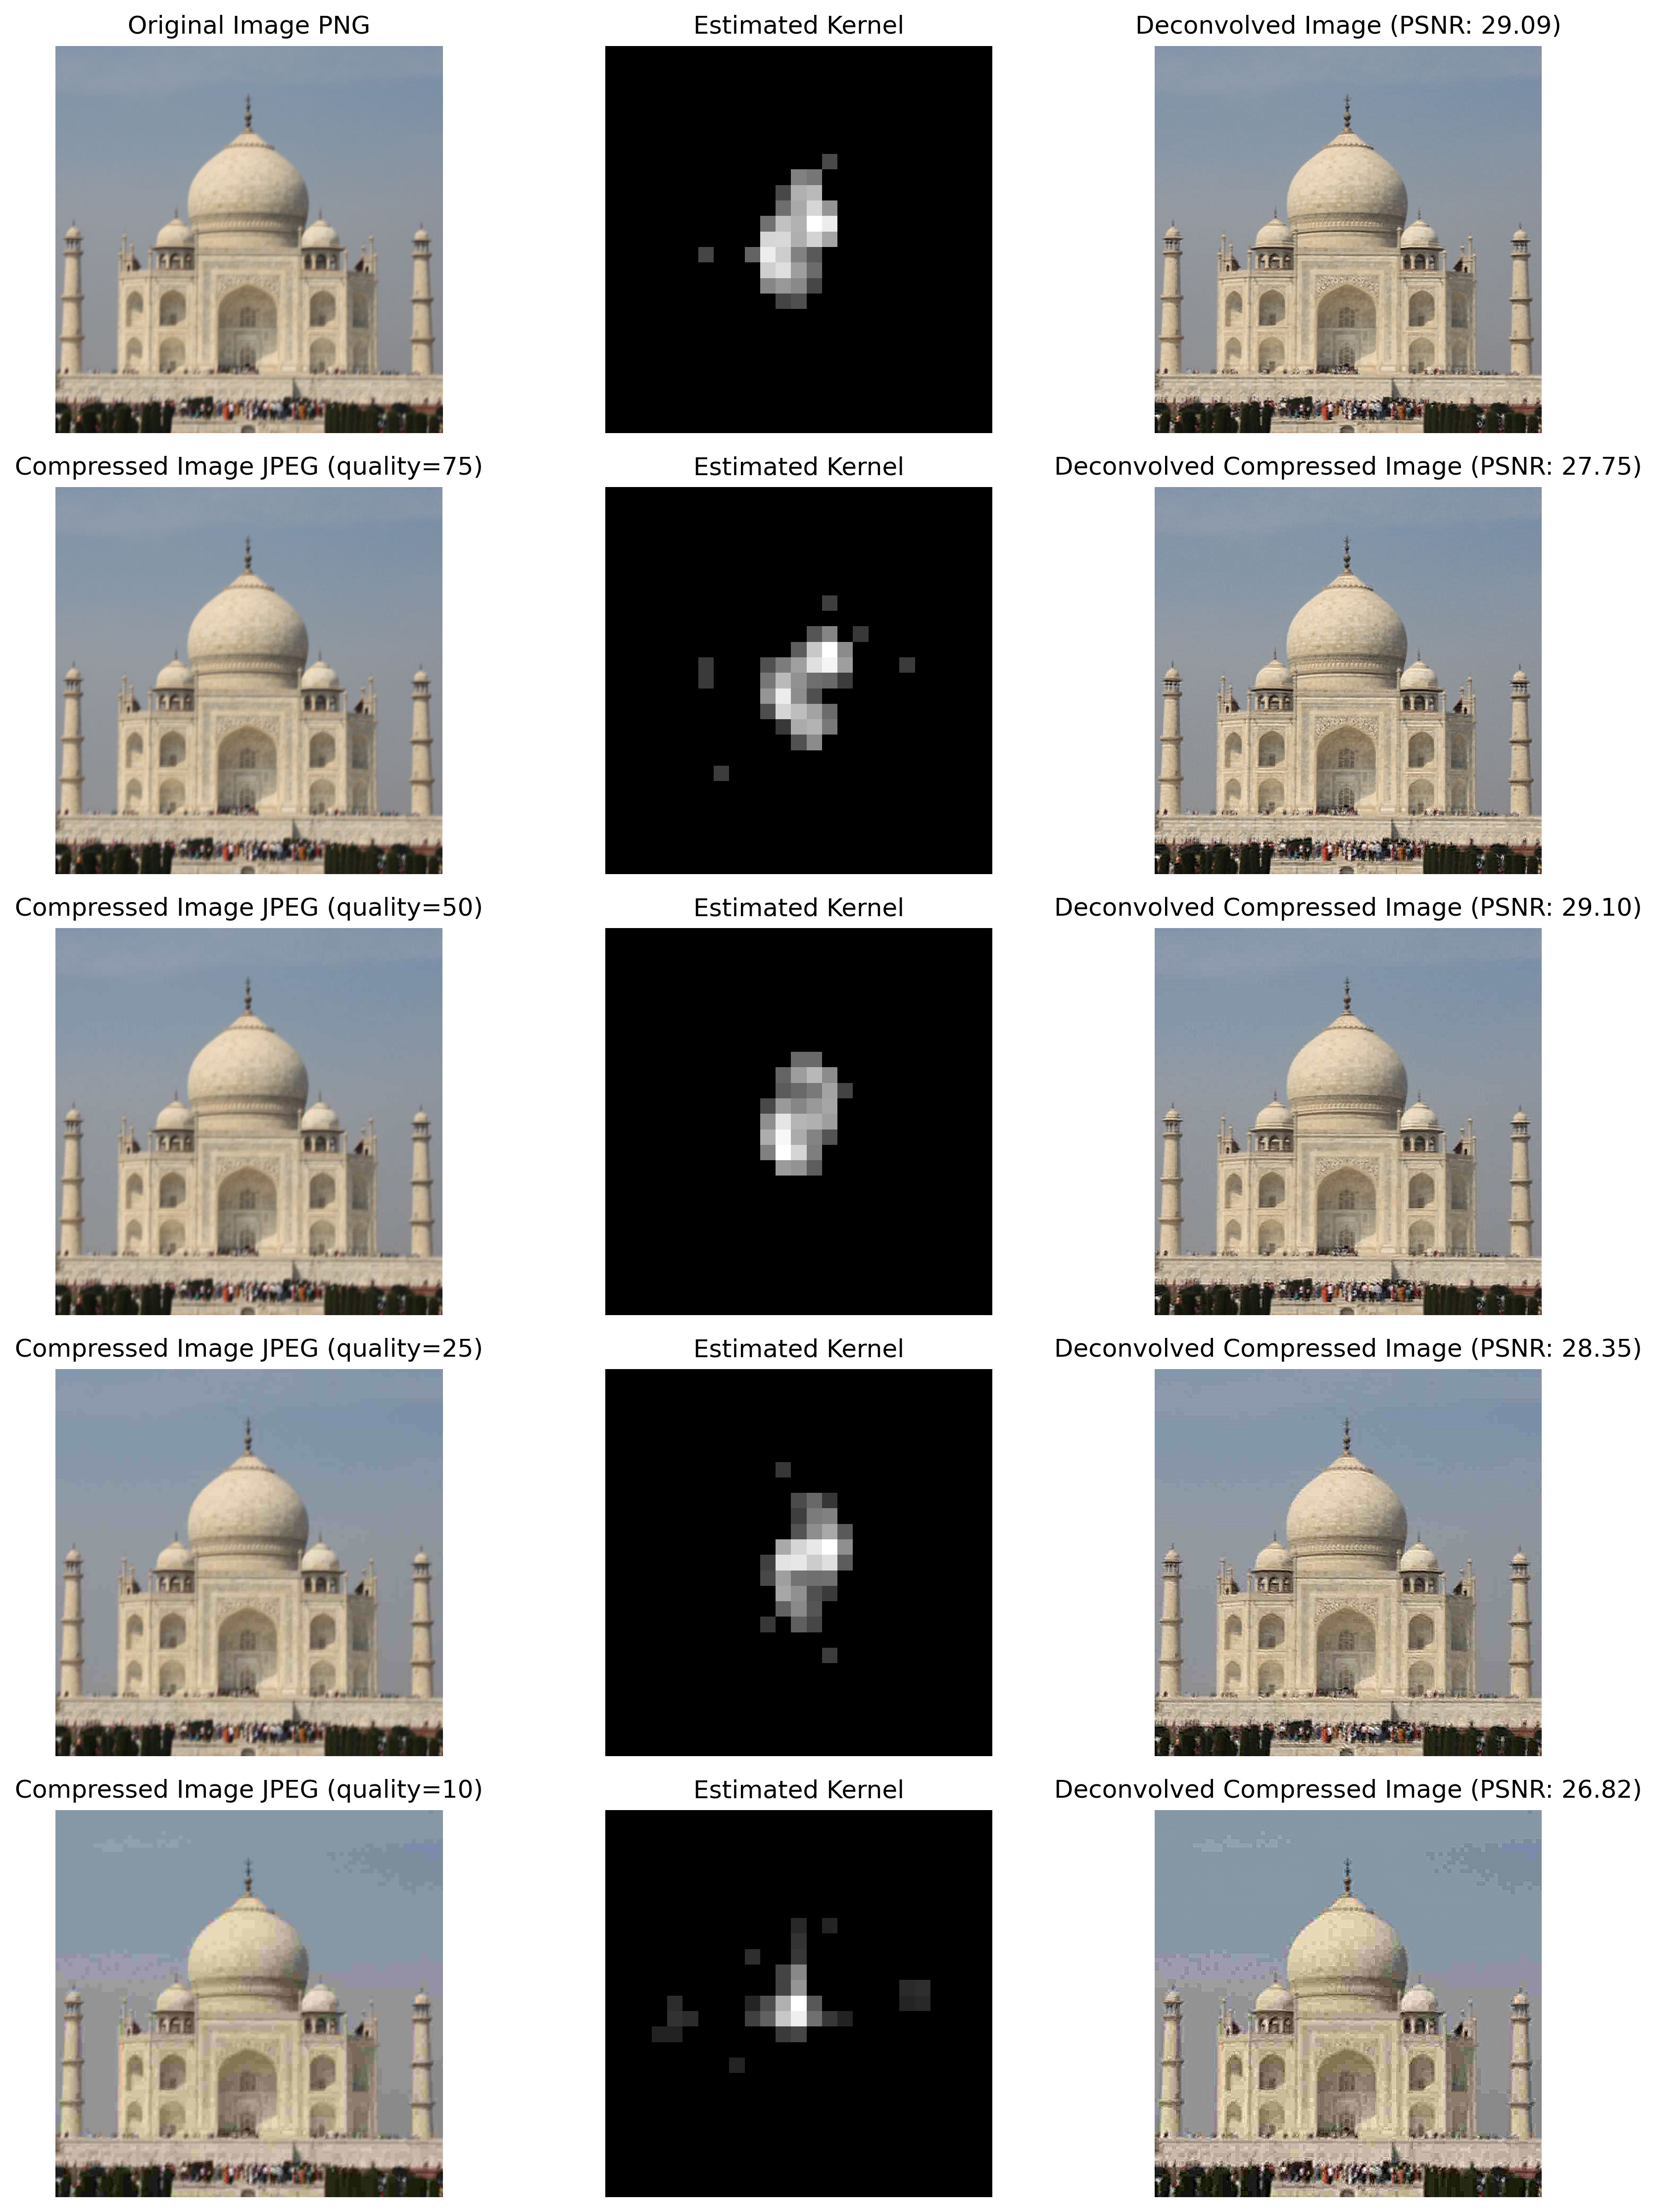
\includegraphics[width=1\linewidth]{../results/compressed_test.png}
    \caption{Comparison of estimated kernels and deconvolved images for different JPEG compression levels (quality factor $Q=75$, $Q=50$, $Q=25$, $Q=10$).}
    \label{fig:jpeg_robustness}
\end{figure}

Figure~\ref{fig:compressed_robustness} illustrates the behaviour of the proposed
pipeline when the blurred image is further degraded by JPEG compression at
different quality factors. The first row corresponds to the reference PNG image:
the estimated kernel is compact and closely matches the ground truth, and the
deconvolved image reaches a PSNR of about $28.9\,\mathrm{dB}$. For moderate
compression levels (quality $75$ and $50$), the JPEG artefacts mainly appear as
weak high–frequency perturbations. The estimated kernels remain very similar to
the PNG case and the PSNR of the restored images decreases only slightly
($27.4$–$28.4\,\mathrm{dB}$), which shows that the kernel estimation and the
TV–deconvolution are fairly robust to mild quantization noise. When the quality
factor is further reduced (quality $25$ and especially $10$), blocking artefacts
and staircase effects become visible in the compressed observations. These
structured artefacts interfere with the whitening step and with the
autocorrelation used to estimate $|\hat h|^2$, leading to slightly more
diffuse kernels and a noticeable but still moderate drop in PSNR (down to
$\approx 27.0\,\mathrm{dB}$ for quality $10$). Overall, the experiments
indicate that the method tolerates typical JPEG compression levels well, and
only starts to degrade for very aggressive compression where the image content
itself is strongly distorted.





\subsection{Limitations of the method}

The experiments above clearly reveal several limitations of the proposed pipeline. First, the entire approach relies on a simplified forward model where the blur is spatially invariant and purely convolutional; this assumption is often reasonable for synthetic motion blur, but it is clearly violated for realistic hand–held camera shakes that combine 3D rotations, depth variations, focus errors and rolling–shutter effects, as observed on the personal RAW images. Second, the Goldstein--Fattal kernel estimator is intrinsically sensitive to measurement noise, to the intrinsic camera blur and to model mismatch: the whitening step amplifies high–frequency perturbations, so the 1D autocorrelations used to recover $|\hat h|^2$ rapidly become unreliable in the presence of strong noise, long motion kernels, severe compression artefacts, or inaccurate support estimation. In turn, any error in the estimated kernel is strongly magnified by the inverse filter during TV--deconvolution, leading to ringing, structured artefacts and a rapid drop in PSNR. Third, the restoration stage itself requires a careful tuning of the hyperparameters $(\lambda,\gamma)$ and of the boundary conditions; circular convolutions are efficient but prone to wrap--around artefacts, whereas symmetric boundaries alleviate these artefacts at the cost of a more complex implementation, and the optimal $(\lambda,\gamma)$ values depend on the noise level, the kernel size and the image content. Finally, the method remains computationally expensive compared to pure non-blind TV deconvolution, since it involves multiple Fourier transforms and a stochastic search over kernel phases, and it cannot exploit semantic priors or large training datasets as modern deep learning approaches do. Overall, these limitations suggest that the technique is best suited to moderately blurred, moderately noisy images where the convolutional model is a good approximation, and that substantial extensions would be required to handle more realistic, heterogeneous degradations.
Compared to alternative Bayesian or MAP-based blind deconvolution methods with richer image priors (e.g., sparsity in learned dictionaries or heavy–tailed gradient models) that jointly estimate the sharp image and the blur kernel, the proposed decoupled approach is simpler and more interpretable but typically less flexible and less robust to severe model mismatch.

\subsection{Suggestions}

Building on the limitations identified above, several directions could be explored to improve the proposed pipeline. A first line of work would be to relax the assumption of a spatially invariant blur and move towards more realistic motion models, for instance by using piecewise-uniform kernels, spatially varying point spread functions, or low-dimensional parametric camera-motion models estimated from the data. On the kernel-estimation side, a particularly weak point of the current implementation is the purely random sampling of Fourier phases: this strategy may miss plausible kernels and tends to be inefficient. A more principled alternative would be to optimise the phase variables explicitly, for example through projected gradient descent on the unit circle, or by embedding the phase estimation in an alternating minimisation scheme that jointly refines the kernel and a provisional sharp image under non-negativity and support constraints. One could also restrict the search to physically plausible motion trajectories (e.g., piecewise-linear paths) and parameterise the kernel by a small number of motion parameters, which would greatly reduce the dimensionality of the phase space.

Concerning the restoration stage, the present work relies on isotropic TV regularisation, which is known to produce staircase artefacts and to oversmooth textures. Several alternative priors could be investigated: higher-order variants such as total generalized variation (TGV) to better preserve smooth intensity ramps, nonlocal or structure–tensor based regularisation to respect oriented textures, or sparse representations in wavelet or learned dictionaries to model fine-scale details more faithfully. One may also replace the quadratic data-fidelity term by more robust losses (such as $L^1$, Huber, or mixed $L^2$--$L^1$ terms) and couple this with automatic hyperparameter selection rules (e.g., discrepancy principles or Stein’s unbiased risk estimates) in order to adapt to different noise statistics without manual tuning.

Finally, a promising perspective would be to hybridise this variational framework with modern data-driven priors. Plug-and-play or RED-type schemes could incorporate powerful pretrained denoisers (BM3D or CNN-based) in place of the TV proximal operator, while unrolled optimisation networks could mimic several iterations of the Goldstein--Fattal + TV-deconvolution pipeline and learn a subset of its parameters from data. Such hybrids would retain the interpretability and control offered by the physical forward model, while benefiting from the expressive power and robustness of learned image priors.


\section{Conclusion}

In this report, we have studied a blind image deblurring pipeline that combines the Goldstein--Fattal kernel-estimation method with a TV-regularised deconvolution solved by the split-Bregman algorithm. On synthetic examples with moderate motion blur and limited noise, the approach proves capable of recovering reasonably accurate kernels and producing sharp restorations, provided that the blur is well approximated by a spatially invariant convolution. The experiments also highlight the importance of implementation choices such as boundary conditions and the tuning of the TV hyperparameters, which have a strong impact on both PSNR and visual quality. However, as soon as the acquisition deviates from the simplified forward model (e.g., complex hand-held camera shake, long motion paths, strong noise or heavy compression), the kernel estimation becomes unstable and the deconvolution step amplifies modelling errors, leading to ringing artefacts and poor restorations. Overall, while the method cannot compete with state-of-the-art deep learning or advanced Bayesian blind deconvolution algorithms on challenging real-world data, it remains attractive as a conceptually simple, interpretable and training-free baseline. The suggested extensions---towards more realistic blur models, more robust priors and possible hybrid variational/learning approaches---constitute natural perspectives for future work on this problem.


\bibliographystyle{plain} 
\bibliography{references}

\end{document}